\capitulo{3}{Conceptos teóricos}


Esta sección aúna los diferentes conocimientos teóricos necesarios para la realización del proyecto. A continuación, y en este orden, se explicarán los algoritmos utilizados, sistemas físicos empleados y  protocolos de comunicación.

\section{Algoritmia}


\subsection{Particle Filter localization}
\label{subsec:PF}

Conocer la localización del agente dentro del mapa es fundamental. No es posible realizar un planeamiento de ruta hacia un destino, como el que realiza el sistema de evasión de obstáculos definiendo unas metas, sin que el agente conozca su posición.
Dada la naturaleza del proyecto, el uso de un GPS para lograr la localización del agente queda descartado. Se requiere de un sistema de localización lo más preciso posible en un interior, por ello se hace uso de un algoritmo basado en probabilidades. 

Los Filtros de Partículas son modelos utilizados para tratar de estimar el estado de un sistema que cambia con el tiempo. 
\\Fue definido como \textit{bootstrap filter} en 1993 por N. Gordon, D. Salmond y A. Smith \citep{art:GSSPF}.  Se trata de un método que pretende implementar filtros bayesianos recursivos, haciendo uso del método de Montecarlo, es decir, realiza repetidas medidas del estado para estimar la variable de interés, en el caso de este proyecto la \emph{localización} del sistema. De esta forma, estimará la posición y orientación de un agente en un entorno, haciendo uso de múltiples hipótesis ponderadas \citep{art:PFTuto}.
Dicha ponderación, peso o probabilidad, se basa en la similitud de la hipótesis, o partícula, con la instancia que representa el agente. 

Para lograr obtener información del entorno, y poder dar una serie de atributos que determinen la afinidad del agente con las partículas, se dispone de los sensores detallados en la subsección \ref{subsec:hcsr04}, que proporcionan la distancia del agente al obstáculo hacia el que se dirige el sensor. 
Haciendo uso de múltiples sensores de distancia, con diferentes orientaciones, se obtienen múltiples distancias a obstáculos, de forma que se reduce la incertidumbre, dado que se dispone de múltiples medidas del entorno que podrán ser comparadas con las del agente. 


Habitualmente, se comienza con una distribución de partículas aleatoriamente dispersas por el mapa, obviamente no se establecen partículas dentro de zonas ocupadas por obstáculos, con una orientación definida. Esto, representa el total desconocimiento de la posición del agente, es decir, todas las hipótesis son equiprobables y por lo tanto la posición del agente es, equiprobablemente, cualquier posición del mapa.

A medida que el agente comienza a  moverse las partículas se mueven en la dirección y orientación que determina el agente, por ejemplo: Si el agente ha rotado 10º y se ha desplazado hacia delante 10 cm, todas las partículas deberán rotar 10º y desplazarse hacia delante 10cm. 
A continuación el agente y las partículas toman medidas de su entorno haciendo uso de los sensores de distancia, en el caso del agente. Cómo calculan las partículas dichas distancias será explicado más adelante.

Una vez realizado el movimiento, la distribución de partículas es remuestreada en base a estimación Bayesiana recursiva, esto es, cuanto se parecen las distancias medidas por el agente a las distancias medidas por cada partícula. O como de parecidas son las hipótesis al estado real del sistema.
El remuestreo, o \textit{resample}, conlleva reducir la población de partículas descartando las menos parecidas, o menos probables. De esta manera al cabo de cierto número de iteraciones la distribución converge hacia la posición real del agente. 

Conviene tener en cuenta que ni los movimientos (tanto de rotación como de traslación), ni las medidas del agente son perfectos, así que se puede añadir cierto \textit{ruido}, distribuido de forma Gaussiana por ejemplo, al movimiento y medidas del agente.
Esto aporta incertidumbre sobre el estado real del agente, lo cual hará que el filtro pueda tardar más iteraciones en converger, pero proporciona un \textit{cubrimiento} más adecuado del estado real del agente.

\subsubsection{Representación del estado}
El \textit{estado} del agente en el caso de este proyecto estará compuesto de las coordenadas del agente en el plano, y su orientación. Se puede representar mediante una n-tupla, donde $n=3$ en este caso, tal que: $[x, y, \theta]$ siendo $x$ e $y$ las coordenadas de posición y $\theta$ la orientación. La altura del agente no es tenida en cuenta, dado que se establece esta como fija, es decir, no existen zonas en las que el agente deba navegar a menor o mayor altura para poder acceder, de manera que no es relevante para el cálculo de la posición conocer esta dimensión.

El \textit{peso} de las partículas, o estimación de la probabilidad de que la partícula sea la ubicación real del agente, es una función de densidad de probabilidad distribuida sobre el espacio de estados, descrito en \citep{wiki:RLtPF}. 
En el \emph{Filtro de Partículas} la variable de interés, la posición del agente, es representada por un set de $M$ partículas en el instante $t = k$, tal que $S^k=[e_j^k,w_j^k]:j=1..M$ tal y como se muestra en \citep{art:PFTuto}. Cada partícula tiene asignado un peso, $w_j^k$ que define la contribución de esa particula a la estimación de la posición.

Aquellas regiones del espacio de estados con una gran cantidad de partículas, se corresponden con zonas en las que hay una alta probabilidad de que el agente se encuentre en ellas. Aquellas zonas con una densidad de partículas baja, representan zonas en las que es improbable que el agente se encuentre.

Claramente es un método que puede ser utilizado como estimador del estado de cualquier sistema.

El algoritmo asume la \textit{propiedad de Markov}\footnote{En un proceso estocástico que cumple la propiedad de Markov, el estado futuro depende únicamente del estado presente, y no de los estados pasados.}, de manera que solo funciona correctamente si el entorno es estático. Por lo general, el agente no tiene información de su localización, así que las partículas se distribuyen de forma uniforme. En implementaciones futuras, se podría hacer uso de SLAM\footnote{Simultaneous Localization and Mapping es una técnica que permite la localización y el mapeo simultáneo de un agente en un entorno desconocido}, para evitar tener que codificar el mapa.

\subsubsection{Actualización de movimiento}
Durante la actualización de movimiento, descrita en \citep{art:PFTuto, art:PFBL}, el agente predice su nueva localización basándose en el movimiento, supuestamente, realizado. Tal y como se ha descrito con anterioridad, si el agente rota 10º en el sentido de las agujas del reloj, todas las partículas rotan en ese mismo sentido el mismo número de grados. 
Sin embargo la capacidad del agente de rotar o trasladarse no es perfecta. Si el sistema de evasión de obstáculos indica al agente que debe rotar $nº$ para dirgirse hacia la meta por un camino seguro, el agente \emph{tratará} de rotar $nº$ pero es muy probable que infra/sobrecorrija.
Si el agente trata de desplazarse en línea recta inevitablemente escorará en una dirección u otra, pese a los sistemas de control embebidos en la controladora de vuelo. 

El movimiento \emph{perfecto} se define de la siguiente manera para el instante de tiempo $t=k$:
\begin{equation}
\label{eq:PFpmovement}
\begin{bmatrix}
x'\\ 
y'\\ 
\hat{\theta'}
\end{bmatrix} = 
\begin{bmatrix}
x + \rho \times cos(\hat{\theta_k})\\
y + \rho \times sin(\hat{\theta_k})\\
\hat{\theta_k}
\end{bmatrix}
\end{equation}
Donde:
\begin{align*}
[x,y,\hat{\theta}]^T &= \text{Posición inicial del agente}\\
\hat{ \theta } &= arctan(\frac{\delta y}{\delta x})\\
[x',y',\hat{\theta'}]^T &= \text{Posición final del agente}\\
\rho &= \sqrt{\Delta x^2 + \Delta y^2}\text{; la distancia a recorrer}
\end{align*}

Aunque para el cálculo de $\hat{\theta}$ el agente dispone de magnetómetro; ver subsección \ref{subsubsec:sensors}
Sin embargo se debe compensar el \emph{ruido} existente en los sensores y sistemas de movimiento, quedando la ecuación \ref{eq:PFpmovement}:
\begin{equation}
\label{eq:PFnmovement}
\begin{bmatrix}
x'\\ 
y'\\ 
\hat{\theta'}
\end{bmatrix} = 
\begin{bmatrix}
x + \rho \times cos(\hat{\theta_k})\\
y + \rho \times sin(\hat{\theta_k})\\
\hat{\theta_k} + f(rand | \mu, \sigma^2)
\end{bmatrix}
\end{equation}
Donde:

\begin{minipage}{\columnwidth}
\begin{center}
\begin{description}
\item $[x,y,\hat{\theta}]^T$ = Posición inicial del agente
\item $\hat{ \theta }$ = $arctan(\frac{\delta y}{\delta x})$
\item $[x',y',\hat{\theta'}]^T$ = Posición final del agente
\item $\rho$ = $\sqrt{\Delta x^2 + \Delta y^2} * f(rand | \mu, \sigma^2)$; la distancia a recorrer \textbf{añadiendo ruido} dado por una distribución normal
\item $\mu$ = $0.0$; se desea un valor aleatorio dentro de una gaussiana con centro en 0.0
\item $\sigma$ = Errores de los sensores o sistemas de movimiento
\end{description}
\end{center}
\end{minipage}


\noindent El ruido, como puede verse en la ecuación \ref{eq:PFnmovement}, se genera mediante una función de distribución normal, como la detallada en la ecuación \ref{eq:gaussian}, con centro en $0.0$ de manera que se pueda infra/sobrecorrejir el movimiento.


De forma inevitable, las partículas que componen el filtro divergirán como consecuencia de la actualización de movimiento aplicando la ecuación \ref{eq:PFnmovement}. Por ello es necesario tomar medidas del entorno.

\subsubsection{Actualización de sensores}
Cuando el agente toma medidas a través de sus sensores, actualiza la distribución de partículas de forma ponderada, tal y como se describe en \citep{art:PFTuto, art:PFBL}, es decir, en base a la probabilidad de que una partícula se corresponda con el estado actual del agente, de manera que aquellas que más afinidad presentan en sus mediciones, serán tenidas en cuenta más a menudo que aquellas que no se parezcan al agente.

Para ello, se calcula para cada partícula la probabilidad, $x_j^{k}$ de ser la posición real del agente basándose en el estado que esta representa, y haciendo uso de una función de distribución normal, o Gaussiana:

\begin{equation}
\label{eq:gaussian}
x_j^{k+1} = f(x|\mu, \sigma^2)=\frac{1}{\sqrt{2\pi \sigma^2}}e^{-\frac{(x-\mu)^2}{2\sigma^2}}
\end{equation}

Donde:
\begin{align*}
\mu &= \text{Distancias de la partícula a los diferentes obstáculos.}\\
\sigma &= \text{Ruido del sistema de sensores.}\\
x &= \text{Distancias reales obtenidas por los sensores del agente.}
\end{align*}

Cabe destacar, que la probabilidad $x_j^{k+1}$ tiene en su superíndice $k+1$, determinando este el instante de tiempo siguiente, es decir la probabilidad de la partícula $j$ \textbf{después} de haber realizado el movimiento.

Se le asignará a cada partícula un peso, proporcional a la probabilidad de tratarse de la ubicación del agente:
\begin{equation}
w_j^{k+1}=w_j^{k}*x_j^{k+1}
\end{equation}

Dicho peso será normalizado de la forma habitual mediante: 

\begin{equation}
w_j^{k+1}=\frac{\tilde{w}_j^k}{\sum_{j}^M \tilde{w}_j^k}
\end{equation}

Donde $\tilde{w}_j^k$ es la medida de peso de una partícula $j$ en el instante de tiempo $k$, antes de ser normalizado.


\subsubsection{Remuestreo}
Una vez que se han obtenido los pesos, el algoritmo deberá generar un nuevo set de partículas a partir del anterior, teniendo en cuenta el peso de cada partícula. Es decir, si se deben generar $N$ nuevas partículas, el algoritmo deberá escoger de entre el set $M$ de partículas, dando mayor prioridad a aquellas que tengan mayor peso. Cabe destacar, que el proceso de selección ha de ser con reemplazo, de manera que puede seleccionarse múltiples veces la misma partícula. 

De esta forma se genera un nuevo set de partículas $M_{k+1}$, en el que la mayor parte de las partículas se encontrará en aquellas posiciones que proporcionen medidas parecidas a las obtenidas por el agente real.


\subsection{Campos Potenciales}
\label{subsec:PF}
\setcounter{equation}{0}
A la hora de lograr una navegación segura en un entorno determinado, es necesario implementar un sistema de evasión de obstáculos. \\Introducido por Oussama Khatib en 1986 \citep{art:Khatib}, el algoritmo de Campos Potenciales aporta una manera de evitar colisionar con los diferentes obstáculos existentes.\\ Se basa en la idea de que el agente se mueve en un campo de fuerzas. 
La posición que debe alcanzar, su meta o destino, se presenta como una fuerza de atracción, y los obstáculos como fuerzas repulsivas. 
Los diferentes vectores fuerza, determinan la dirección y magnitud de la fuerza atrayente o repulsora.

Sea $q$ la posición actual del agente, considerada como una partícula moviéndose en un espacio n-dimensional $R^n$. Por simplicidad, se considera la posición como una tupla, esto es, bidimensional, tal que $q = (x,y)$. El campo potencial en el que se encuentra el agente es una función escalar $ U(q):R^2\rightarrow R $, generado por la superposición de los campos atrayentes $U_{att}$ y repulsores $U_{rep}$:
\begin{equation}
U(q) = U_{att}(q) + U_{rep}(q)
\label{equation:Uq}
\end{equation}

Por supuesto, la suma de todos lo campos repulsores $U_{rep}$ generan un vector repulsor, que sumado al de atracción puede determinar la necesidad de acercarse o alejarse de una determinada zona:
\begin{equation}
U(q) = U_{att}(q) + \sum_i{U_{rep_i}(q)}
\label{equation:UqTotal}
\end{equation}

Donde $U_{rep_i}$ representa el campo potencial generado por un obstáculo $i$.

Suponiendo que $U(q)$ es diferenciable, en cada punto $q$, el campo potencial $\nabla(q)$ es un vector que apunta en la dirección que, \textbf{localmente}, incrementa $U(q)$. \\De esta forma, si el potencial de atracción en la meta se considera 0 y a medida que el agente se distancia de ella, se incrementa, se puede establecer, teniendo en cuenta el potencial de repulsión producido por los diferentes obstáculos, un vector $F(q)$ cuya dirección apunta hacia donde se reduce el potencial $U$, y su magnitud establece la velocidad con que este se reduce:
\begin{equation}
F(q) = F_{att}(q) + F_{rep}(q) = -\nabla U_{att}(q) - \nabla U_{rep}(q)
\label{equation:Fq}
\end{equation}


\textbf{El potencial de atracción} $U_{att}(q)$ se establece como una función cuadrática proporcional a la distancia a la meta. De esta forma crece exponencialmente a medida que el agente se aleja de su destino, y se reduce considerablemente en su cercanía. Así puede ser utilizado como fuente de información para establecer la velocidad de aproximación al objetivo, de forma que el agente no sobreactúe:
\begin{equation}
U_{att}(q) = \epsilon * \delta_{meta}(q)^2
\label{equation:Uatt}
\end{equation}
Donde $\delta$ es la distancia euclidiana desde la posición del agente $q$ a la meta $meta$, y $\epsilon$ es un factor de escalado positivo, que puede utilizarse para ajustar la influencia de la distancia en la velocidad del agente. Y su gradiente negativo: 
\begin{equation}
-\nabla U_{att}(q) = -\epsilon * (q - q_{meta})
\label{equation:dUatt}
\end{equation}
\begin{figure}[H]
	\centering
	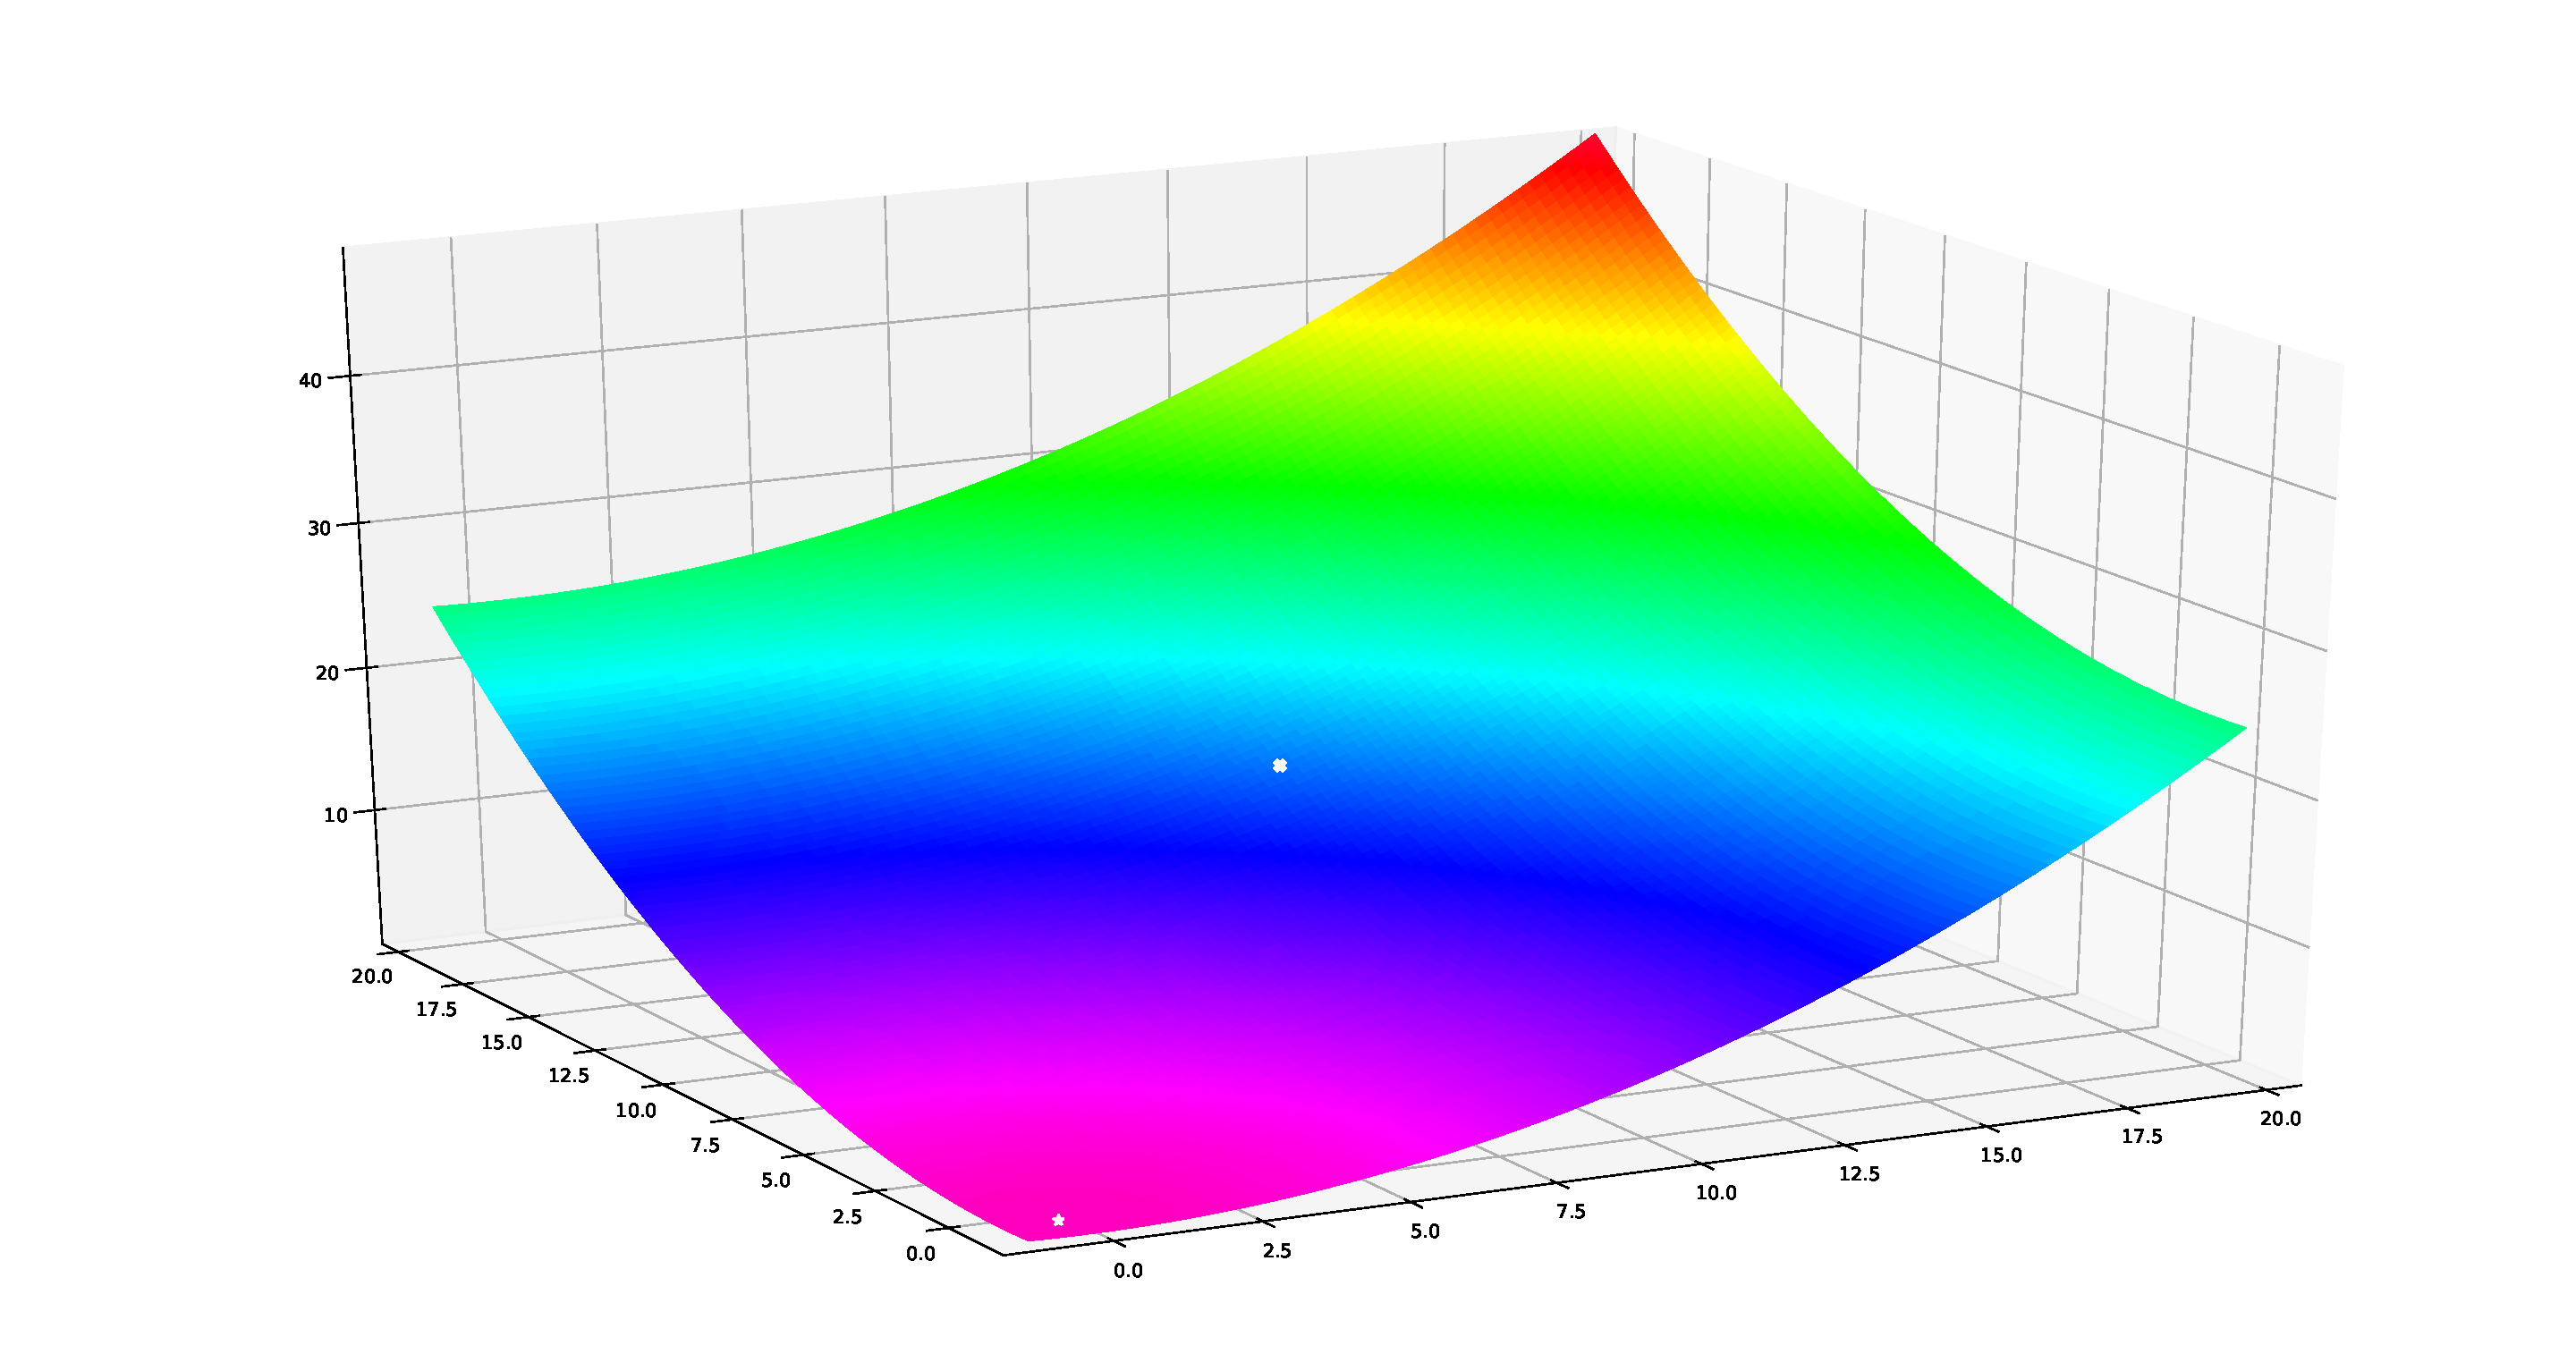
\includegraphics[width=\textwidth]{UattrGradient}
	\caption{Gradiente de Potencial de Atracción.}\label{fig:uattrgrad}
\end{figure}

En la figura \ref{fig:uattrgrad} se ha establecido el agente en el punto $(10,12)$ y la meta en $(0,0)$. Puede verse el efecto del gradiente aplicado.

\textbf{El potencial de repulsión} $U_{rep}(q)$ lo establecen los obstáculos detectados por los sensores del agente. Si se establece una función proporcional a la distancia del agente a los obstáculos, el potencial repulsor crece en la cercanía a estos, y decrece con la distancia. De esta forma un obstáculo lejano al agente no debería presentar ninguna fuerza sobre él:
\begin{equation}
U_{rep}(q) = U = \begin{cases}
0 & \text{ si } \delta > \rho \\ 
\eta * (\frac{1}{\delta_{obs}(q)}-\frac{1}{\rho})^2 & \text{ si } \delta \leq \rho; \delta \neq 0 
\end{cases}
\label{equation:Urepq}
\end{equation}
Donde $\eta$ es un factor de escalado positivo, que permite establecer con qué intensidad se ve afectado el agente por el campo repulsor, $\delta$ es la distancia euclidiana desde la posición del agente $q$ al obstáculo $obs$, y $\rho$ es un factor de escalado positivo, que permite establecer la distancia de influencia de forma proporcional. Y su gradiente
\begin{equation}
-\nabla U_{rep}(q) = \begin{cases} 0 & \text{ si } \delta > \rho \\
\eta * (\frac{1}{\delta_{obs}(q)}-\frac{1}{\rho}) * \frac{1}{\delta_{obs}(q)^2}\frac{q-q_{obs}}{\delta_{obs}(q)} & \text{ si }  \delta \leq \rho; \delta \neq 0  
\end{cases}
\label{equation:dUrepq}
\end{equation}
\begin{figure}[H]
	\centering
	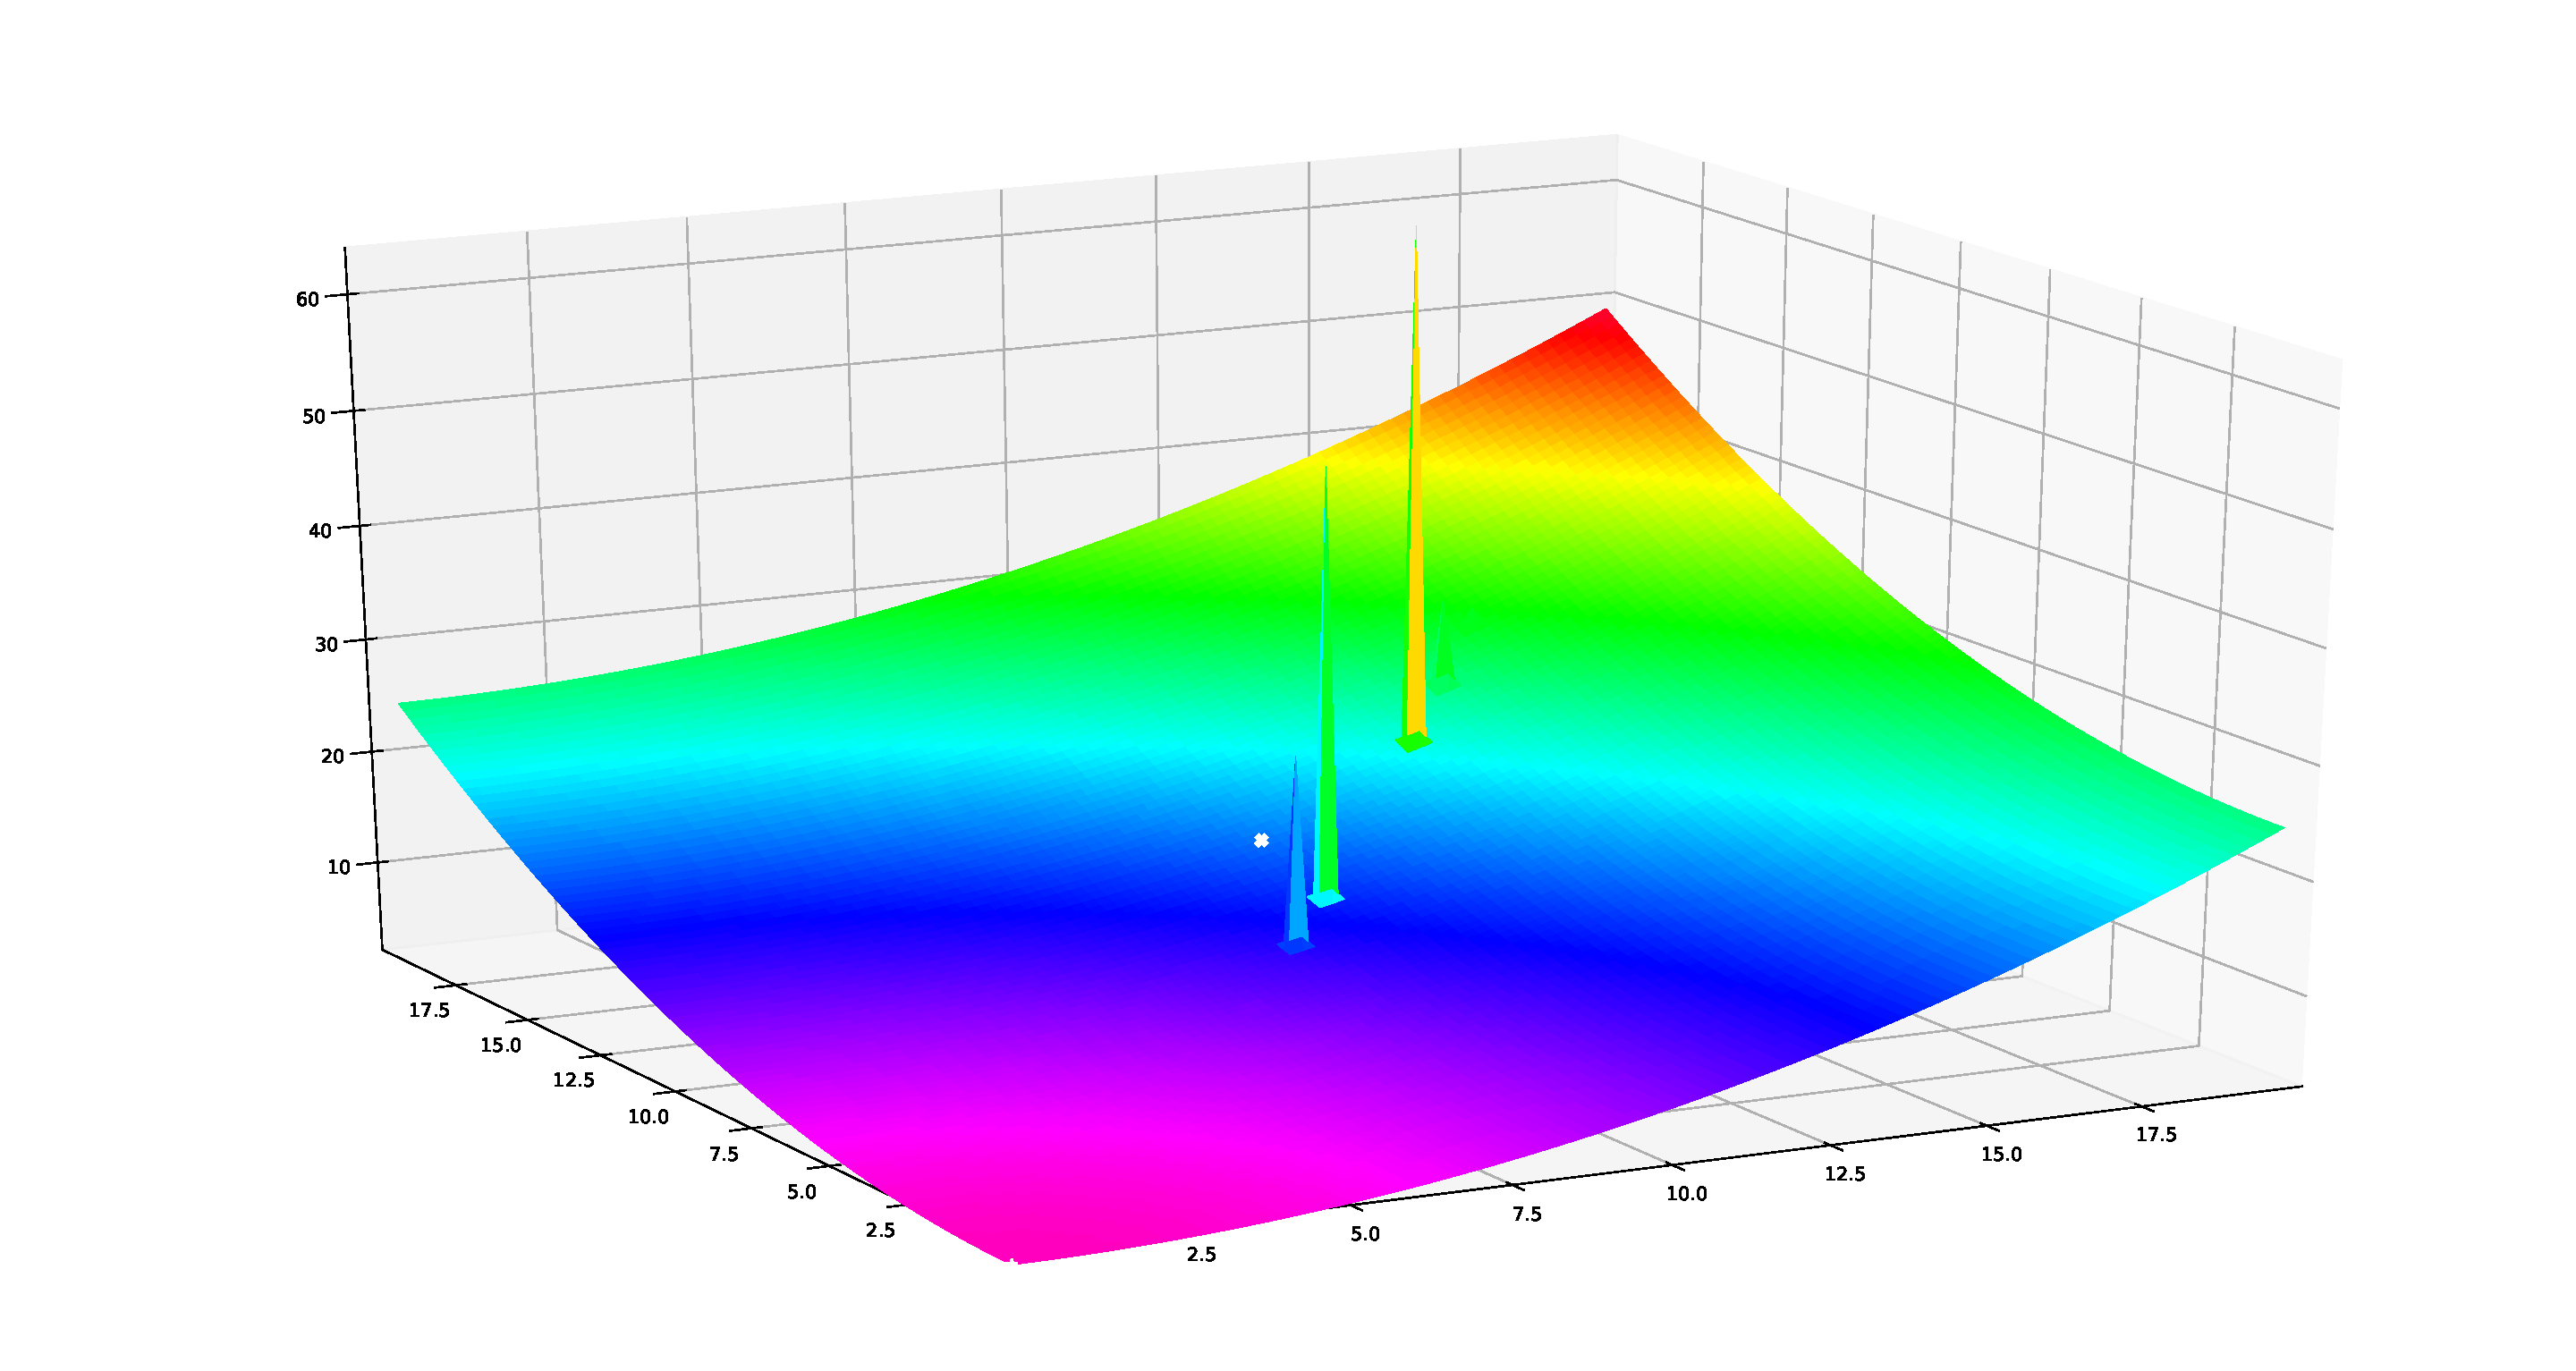
\includegraphics[width=\textwidth]{UrepGradient}
	\caption{Gradiente de Potencial de Repulsión.}\label{fig:urepgrad}
\end{figure}

 En la figura \ref{fig:urepgrad} se ha creado una serie de obstáculos artificialmente para ilustrar el comportamiento del algoritmo. El agente se encuentra en la posición $[10, 12]$, la meta esta establecida en $[0, 0]$ y existen obstáculos en las posiciones $[3, 2], [5, 5], [9, 12], [10, 11]$. El algoritmo no está teniendo en cuenta la fuerza repulsora que representa el obstáculo situado en $[3, 2]$ por encontrarse este demasiado lejos del agente.

 \newpage
\subsubsection{Desventajas}
El algoritmo de campos potenciales se puede llevar a cabo con una implementación simple y eficiente haciendo uso de Numpy, dado que se puede crear una representación matricial del plano en que se desplaza el agente, que contenga los diferentes potenciales en cada posición. 
Esto hace sencillo realizar cálculo vectorizado sobre las matrices. \\Sin embargo, tiene ciertas desventajas, tal y como publicaron Borenstein y Koren \citep{art:BorensteinLims}, que lo han hecho, cuanto menos, inútil para las necesidades de este proyecto:
\begin{itemize}
\item Es un algoritmo basado en descenso de gradiente, y como tal puede quedar \textit{atascado} en mínimos locales. Estos mínimos pueden encontrarse en zonas que contengan obstáculos en forma cóncava o de caja abierta, tal como se ilustra en la figura \ref{fig:localmin}.
\begin{figure}[H]
	\centering
	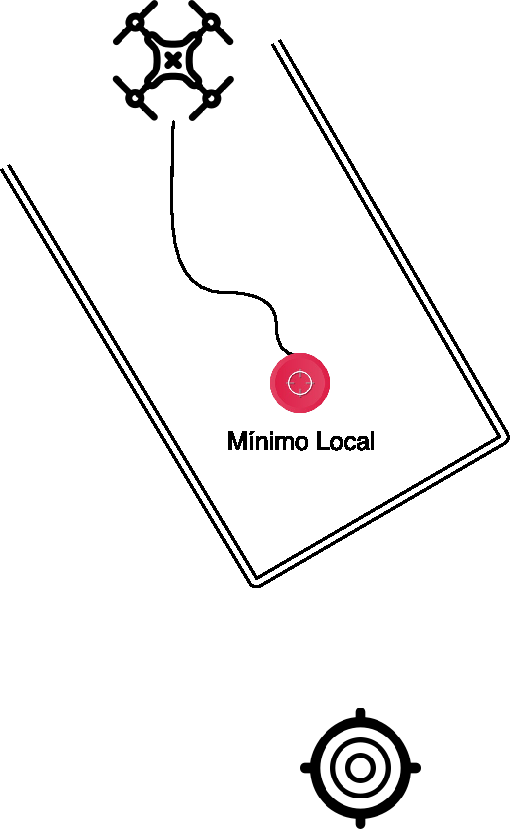
\includegraphics[width=0.5\textwidth]{localmin}
	\caption{Mínimo local en zonas convexas.}\label{fig:localmin}
\end{figure}
\item \label{subsec:PFlims} De encontrarse en un espacio con forma de corredor o pasillo, cualquier acercamiento hacia las paredes ocasionará una corrección en el sentido opuesto al campo repulsor, lo cual puede ocasionar un movimiento oscilatorio si dicha corrección supone aproximar el agente a la pared opuesta, tal y como se ilustra en la figura \ref{fig:corridoroverc} extraída de \citep{art:BorensteinLims}.
\begin{figure}[H]
	\centering
	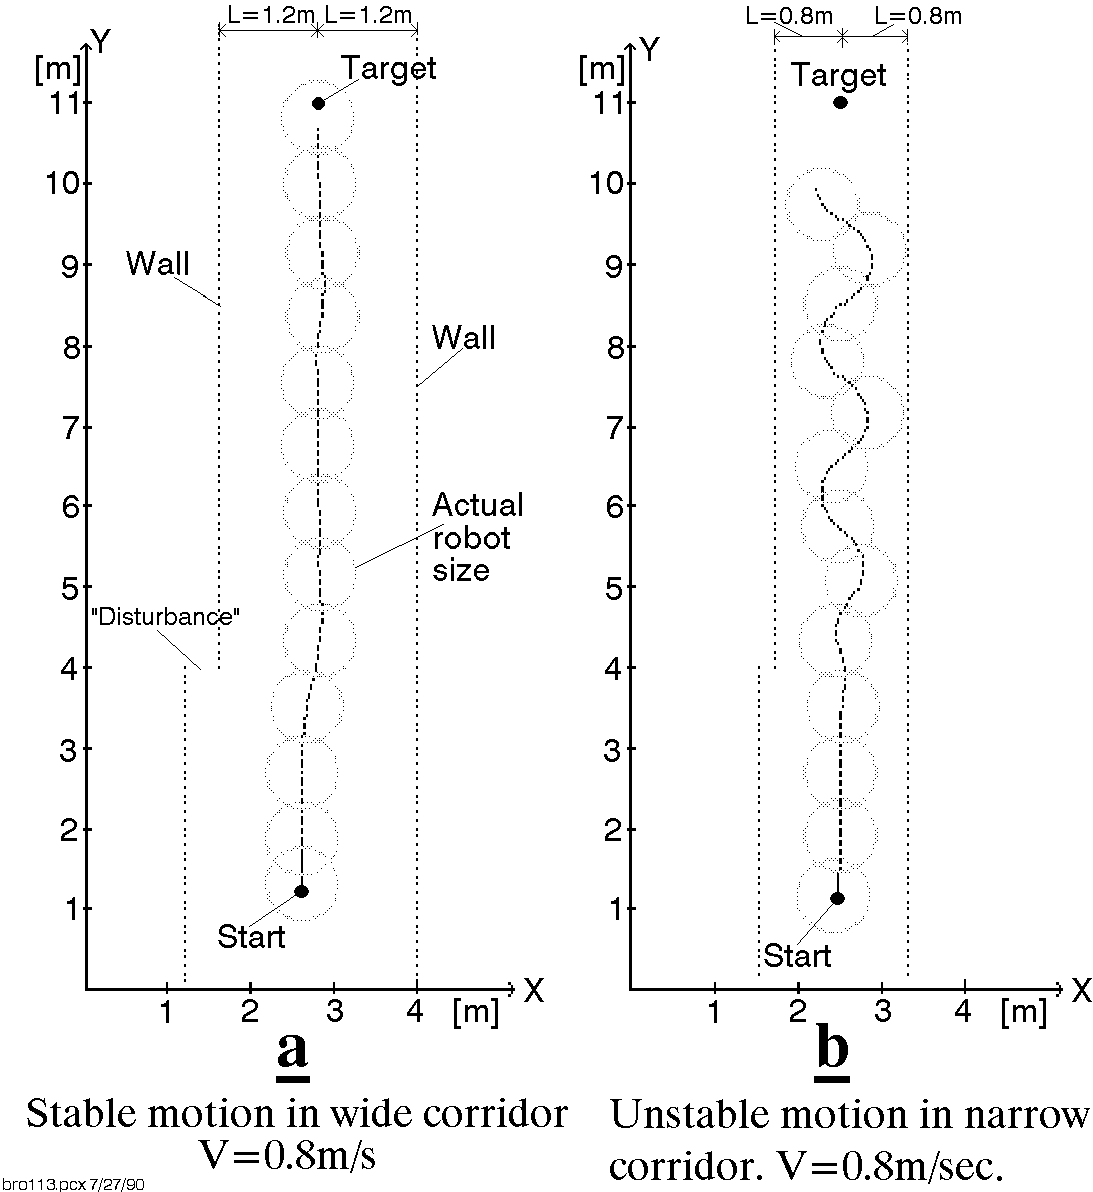
\includegraphics[width=0.9\textwidth]{corridoroverc}
	\caption{Movimiento oscilatorio en corredores estrechos.}\label{fig:corridoroverc}
\end{figure}
\item Alta complejidad computacional pese a poder modelarse como calculo vectorizado, requiere de muchas más operaciones que otros métodos más avanzados.
\item No funciona correctamente con agentes que se desplazan a alta velocidad. 
\item Al realizar la adición de todos los campos potenciales, tanto repulsores como atrayente, se produce una gran pérdida de información sobre la distribución local de los obstáculos.
\end{itemize} 

Por estos motivos, se ha desechado el algoritmo de Campos Potenciales como sistema de evasión de obstáculos, y se ha pasado a un modelo más avanzado basado en un plano cartesiano, conocido como \textit{Vector Field Histogram} y detallado en el apartado \nameref{subsec:VFH}. 

\subsection{Vector Field Histogram}
\label{subsec:VFH}
El Vector Field Histogram, o Histograma de Campos Vectoriales, \textit{VFH} de aquí en adelante, fue introducido por Borenstein y Koren en el año 1991 \citep{art:BorensteinKorenVFH, art:BorensteinKorenFMCE}. Permite la detección de obstáculos y su evasión mediante el control de la dirección y velocidad del agente en tiempo 
real.

Para ello realiza una representación del entorno del agente en forma de histograma. Dicho entorno, llamado \textit{Región Activa $C*$} se representa como una \textit{ventana} que se desplaza con el agente en el centro. Se trata un algoritmo de búsqueda local, sin embargo se ha mostrado que suele producir rutas cercanas al óptimo, aunque en el caso de este proyecto no es relevante, dado que la intención es que se exploren todas las zonas del entorno.

Es un algoritmo más robusto, dado que presenta cierta insensibilidad a lecturas erróneas, y eficiente que el algoritmo de Campos Potenciales explicado en la subsección \ref{subsec:PF}. 

Se compone de tres partes: 
\begin{enumerate}
\item Red Cartesiana de Histogramas: Derivado del concepto de \textit{malla de certidumbre} propuesto por Moravec y Elfes en 1985 \citep{conf:CertainityGrid}  en la universidad de Carnegie Mellon. Se construye un plano cartesiano representando el entorno cercano del agente. Por \textit{cercano}, se entiende una distancia que los sensores de distancia puedan abarcar, dado que no tendría sentido tratar de computar zonas inalcanzables en un momento determinado. Dicho plano será representado como un histograma, y de ahí su nombre habitual \textit{Cartesian Histogram Grid}. Ver subsección \ref{subsubsec:CHG}.
\item Histograma Polar: Una representación unidimensional, obtenida a partir de una reducción de la Red Cartesiana definida en el punto anterior. Se compone de $n$ sectores angulares $k$, de anchura $\alpha$, de forma que $n * \alpha = 360; n \in \mathbb{Z}$. Dichos sectores $k$ contienen un valor $h_k$ que representa la densidad de obstáculos, \textit{Polar Obstacle Density} o \textit{POD} de aquí en adelante, contenida en él. Ver subsección \ref{subsubsec:PH}.
\item Capa de salida: Representa el resultado del algoritmo. A partir del POD, se obtienen los posibles \textit{valles}\footnote{Así denominados por su representación en forma de histograma} candidatos existentes entre obstáculos, y se elige el que más se aproxime a la dirección de la meta establecida. Finalmente, entrega los valores de cambio de dirección necesario en cada momento. Ver subsección \ref{subsubsec:OL}.
\end{enumerate}

\subsubsection{Cartesian Histogram Grid}
\label{subsubsec:CHG}
Se modela el espacio cercano al drone en forma de malla. En cada celda $(i,j)$ de esa malla se encuentra un valor $c_{i,j} \in \mathbb{Z}$ que establece la certeza de la existencia de un obstáculo. La cantidad de celdas existentes en la malla se establece en función de los límites del sensor, y teniendo en cuenta que es necesario establecer una precisión $c$, por ejemplo: Si se dispone de un sensor con un rango de medidas de hasta 400 cm se puede crear una malla de $81\times 81$, suponiendo que cada celda tenga un tamaño de $c=5$, $5 \times 5cm$, en cuyo centro se encuentra el drone, dejando 40 filas y columnas a cada lado. Y estableciendo así, un perímetro de medidas de 200 cm en cada dirección desde el drone. De esta forma se consigue una precisión de $\pm5\text{cm}$

Dicho valor se obtiene de la lectura proporcionada por el sensor de distancia, en este caso un sonar, y se establece en el centro del ángulo de barrido del sonar, ver subsección \ref{subsec:hcsr04}. 
La eficiencia superior de este algoritmo se basa precisamente en incrementar el valor $c_{i,j}$ de únicamente una celda con cada medida. Dicha celda $(i,j)$ se encuentra a una distancia de $R = \frac{\delta_{obs}q}{c}$ celdas y en la bisectriz del ángulo barrido por el sonar.
Si bien está solución puede parecer una simplificación del problema, se llega a generar una distribución probabilística tomando múltiples medidas de forma continua mientras el agente se desplaza por el entorno. Por tanto, la misma celda, cercana a un obstáculo, y sus vecinas serán incrementadas repetidas veces, tal y como se muestra en la figura \ref{fig:histog1}, extraída de \citep{art:BorensteinKorenVFH}.
 \begin{figure}[H]
	\centering
	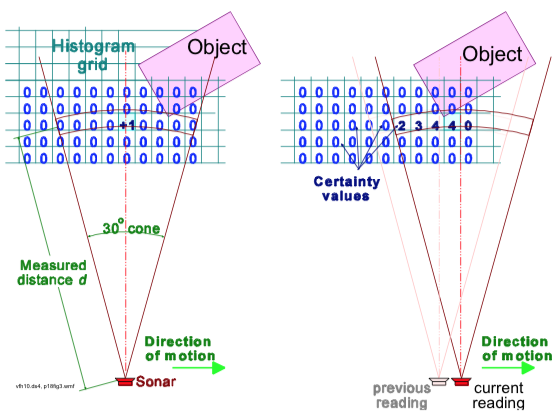
\includegraphics[width=0.9\textwidth]{HistoG1}
	\caption{Distribución Histográmica de Probabilidades.}\label{fig:histog1}
\end{figure}

\subsubsection{Polar Histogram}
\label{subsubsec:PH}
A partir de las medidas obtenidas en el Histogram Grid, se realiza la primera reducción de información para construir un Histograma Polar. Para ello, los contenidos de la región activa $C*$ son tratados como un \textit{vector de obstáculos} cuya dirección está definida por la dirección $\beta$ de la celda en cuestión al centro del agente \textit{VCP}\footnote{El VCP o \textit{Vehicle Center Point} se define como el centro geométrico del vehículo. En nuestro caso, al tratarse de un drone, se considera el centro del mismo como VCP}, y que viene definida por la función:
\begin{equation}
\label{equation:ObsAgAng}
\beta_{i,j}= tan^{-1} \frac{y_i - y_0}{x_i - x_0}
\end{equation}

La ecuación \ref{equation:ObsAgAng} devuelve un valor $\beta \in [-\frac{\pi}{2}, \frac{\pi}{2}]rad$. Al hacer uso de Numpy, es sencillo calcular los ángulos en los que se encuentra cada celda de la región activa $C*$ con respecto al agente que se encuentra en su centro, de forma vectorizada. Tal y como puede verse en la figura \ref{fig:histog2}.
 \begin{figure}[H]
	\centering
	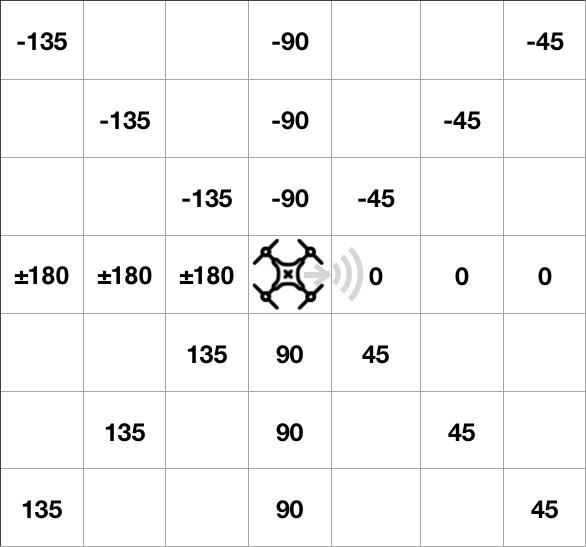
\includegraphics[width=0.9\textwidth]{HistoG2}
	\caption{Angulos relativos al VCP del drone.}\label{fig:histog2}
\end{figure}

Nótese que para llevar a cabo la obtención de estos ángulos \textbf{no} se ha hecho uso de la función \textit{arctan} disponible en Numpy, dado que esta devuelve valores, en radianes, pertenecientes al 1º y 4º cuadrante únicamente. En su lugar, se ha utilizado la función \textit{arctan2}, que tiene en cuenta el signo de las componentes del vector dirección $ [y_i - y_0 , x_i - x_0]$ resultante, de forma que devuelve el ángulo de giro, sea en sentido horario (valores positivos) o antihorario (valores negativos), más corto posible\footnote{Obviamente es lo deseable, no sería eficiente realizar un giro de 225º en el sentido de las agujas del reloj, cuando uno de 135º en el sentido contrario a las agujas del reloj bastaría.}.


La magnitud de cada zona es entonces calculada de la siguiente forma:

\begin{equation}
\label{equation:mij}
m_{i,j} = c*_{i,j}^2 * (a-bd_{i,j})
\end{equation}
Donde: 
\begin{align*}
m_{i,j}  &= \text{Magnitud de obstáculos en la celda $(i,j)$}\\
c*_{i,j} &= \text{Certidumbre de obstáculo en la celda, en la región activa, $(i,j)$}\\
\text{y:} \\
a &= \text{Representa la fuerza con que un obstáculo afecta al drone}\\
b &= \text{Representa la distancia desde la que un obstáculo afecta al drone}\\
\text{son positivos}
\end{align*}

El plano es convertido en una secuencia de sectores que cubren los 360º. Se definen, por tanto, $n \in \mathbb{Z}$ sectores $k$ de amplitud $\alpha$, por ejemplo $n=72; \alpha=5$. Y se distribuyen las medidas tomadas anteriormente en los diferentes ángulos relativos al VCP del drone, en los sectores $k_i$ correspondientes, véase la ecuación \ref{equation:betatok} 
\begin{equation}
\label{equation:betatok}
k =\frac{\beta_{i,j}}{\alpha}
\end{equation}

con un valor $h_k$, véase la ecuación \ref{equation:sumcij}, de densidad de obstáculos en ellos:
\begin{equation}
\label{equation:sumcij}
h_k = \sum m_{i,j}
\end{equation}

Dada la discretización de los datos obtenidos del Polar Histogram el resultado, al realizar esta conversión y al obtener el sumatorio $h_k$ de todos los valores pertenecientes a un sector $k$, puede parecer que el histograma varía de forma muy repentina entre dos sectores. Por ello se aplica una función de suavizado. 
Según J. Borenstein y Y. Koren en \citep{art:BorensteinKorenVFH}, la función de suavizado utilizada se corresponde con: 
\begin{equation}
\label{equation:PODsWRONG}
h'_k = \frac{h_{k-l} +2h_{k-l+1} + ... + lh_k + ... + 2h_{k+l-1} + h_{k+l}}{2l+1}
\end{equation}
Donde $l$  es una constante positiva a la que se le ha dado un valor de $5$. 

Sin embargo, existe una errata en el artículo publicado, y la ecuación \ref{equation:PODsWRONG} no es consistente, i.e:
La función de suavizado parece poder expresarse de forma general tal que:
\begin{equation}
\label{equation:PODsWRONGgen}
h'_k =\frac{1}{2l+1} \sum_{n=-l}^{l} (l-  |n| +1)*h_{k+n}
\end{equation}
ej: $l = 5$ $ h'_k = \frac{1h_{k-5} +2h_{k-4} + 3h_{k-3} + 4h_{k-2} + 5h_{k-1} + \textbf{6}h_k + ... + 2h_{k+l-1} + h_{k+l}}{2l+1} $

Como puede verse, el valor central $ 6h_k $ correspondiente a $n=0$, no coincide con la posición dada para ese valor de $n$ en la función de suavizado propuesta por J. Borenstein y Y.Koren, donde el coeficiente que multiplica a $h_k$ es igual a $l$ en lugar de $l+1$.

Por ello, se ha hecho uso de una función de suavizado preexistente en SciPy, en concreto en el módulo \textit{signal}. Se ha elegido la función de Hann, llamada así por el meteorólogo asutriaco Julius van Hann. Se conoce a esta función por el nombre de Campana de Coseno, y se define por la ecuación \ref{equation:hannWindow}.
\begin{equation}
\label{equation:hannWindow}
w(n)=0.5 - 0.5 cos\frac{2 \pi n}{M-1}\\
0 \leq n \leq M-1
\end{equation}
Donde $M$ es el número de puntos en la ventana de salida. En este caso tomará el valor de $l$.

De esta forma, de obtener un histograma de $n$ sectores con valores $h_k$ posiblemente dispares sectores $k$ contiguos, se pasa a obtener un histograma suavizado, que será de mayor utilidad para el sistema de evasión de obstáculos. Véase la figura \ref{fig:PODandsPOD}

 \begin{figure}[H]
	\centering
	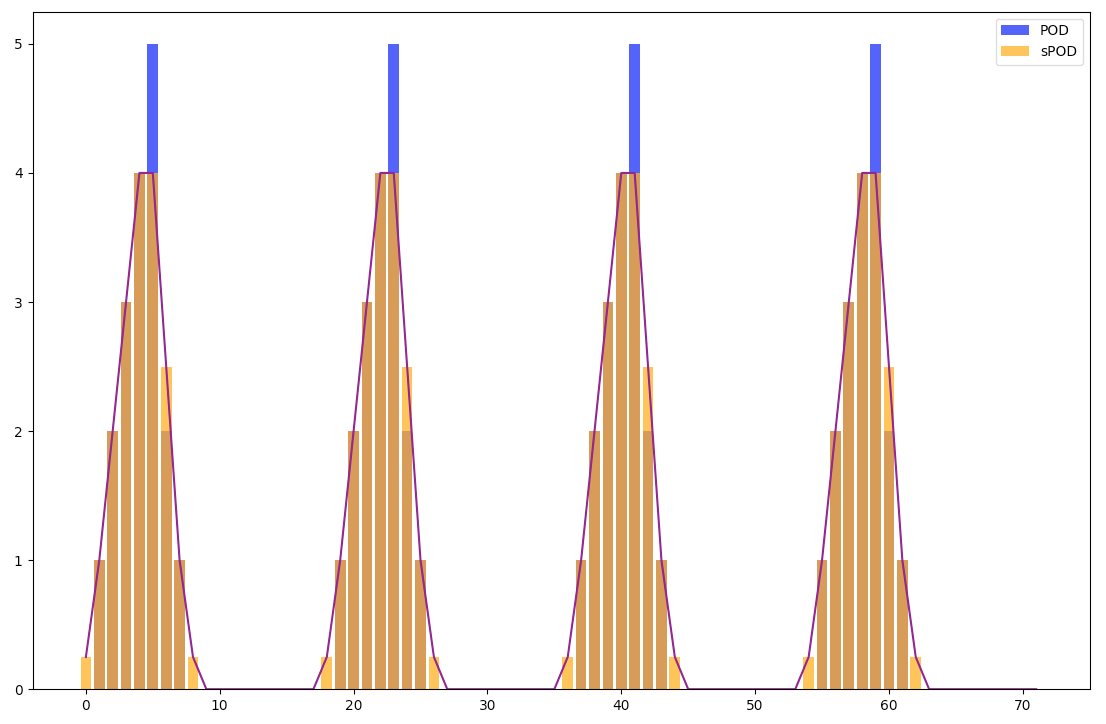
\includegraphics[width=0.9\textwidth]{PODandsPOD}
	\caption[POD vs smoothPOD.]{En azul Polar Obstacle Density(POD). En naranja el suavizado de este (sPOD).}\label{fig:PODandsPOD}
\end{figure}

\subsubsection{Output Layer}
\label{subsubsec:OL}
En el último estadio del algoritmo VFH, se computa el ángulo de giro $\theta$ que se debe aplicar al drone para dirigirlo, por una ruta segura, hacia el destino establecido.
Una vez obtenido el \textit{Polar Obstacle Density}, y aplicado el suavizado correspondiente, se puede determinar en que sectores $k$ existe un \textit{valle}. Se define un \textit{valle candidato} como una zona, compuesta de varios sectores por los que es seguro navegar, es decir, están libres de obstáculos o su densidad de obstáculos esta por debajo de cierto umbral. 

Por lo general se crean dos o más valles candidatos al analizar el entorno, de forma que es necesario elegir aquel que dirigirá al drone en dirección al destino $k_{targ}$. Una vez escogido el valle, se deberá seleccionar el sector $k$ idóneo. Para ello se mide el tamaño del valle, es decir el número de sectores consecutivos por debajo del umbral que lo componen, de esta forma se distinguen dos tipos de valles, amplios y estrechos. 
Los valles amplios son el resultado de espacios grandes entre obstáculos, o de situaciones en las que únicamente existe un obstáculo lo suficientemente cerca del drone. Por \textit{grande} se define una constante $s_{max}$ que determina el número de sectores $k$ que componen un valle amplio.

El sector más cercano a $k_{targ}$ y por debajo del umbral se denomina $k_n$, y representa el \textit{borde cercano} del valle. El más lejano $k_f$ que en el caso de los valles amplios coincide con el valor de $s_{max} + k_n$.  Véase la figura \ref{fig:wvalley1}.

El sector que debe seguir el drone para dirigirse hacia $k_{targ}$ sin peligro, se denomina $\theta_{yaw}$, y su valor es la media de los valores de $k_n$ y $k_f$, como puede verse en la ecuación \ref{equation:thetaYaw}.

\begin{equation}
\theta_{yaw} = \frac{k_n + k_f}{2}
\label{equation:thetaYaw}
\end{equation}


 \begin{figure}[H]
	\centering
	\includegraphics[width=0.9\textwidth]{wideValley1}
	\caption[Valles estrechos y anchos.]{Valle ancho encontrado entre el obstáculo, a la derecha, y un espacio abierto, a la izquierda.}\label{fig:wvalley1}
\end{figure}


Sin embargo, la ecuación \ref{equation:thetaYaw} presenta un comportamiento errático cuando el destino se encuentra dentro de un valle, dado que se establece $\theta_{yaw}$ como la media entre los sectores cercano y lejano, al encontrarse la meta en un sector dentro del valle, el drone no se aproxima a ella sino que realiza círculos cada vez más cerrados hasta llegar al destino, como puede verse en la figura \ref{fig:nToWFOV}

 \begin{figure}[H]
	\centering
	\includegraphics[width=0.7\textwidth]{narrowToWideVfov}
	\caption[Movimiento circular del agente.]{Movimiento circular al encontrarse $k_{targ}$ en un sector seguro por ecuación \ref{equation:thetaYaw}}\label{fig:nToWFOV}
\end{figure}

La intención tras la ecuación \ref{equation:thetaYaw} es la navegación segura en entornos con obstáculos cercanos, ya que aporta la cualidad de escoger la zona central entre dos obstáculos para usarla como zona de navegación segura\footnote{Una cualidad de la que el algoritmo de campos potenciales adolecía, generando movimientos oscilatorios en espacios cerrados, como ya se vió en la subsección \ref{subsec:PFlims}.}. Además en el momento en que la posición del drone sea intermedia entre dos obstáculos, la ecuación \ref{equation:thetaYaw} dará como resultado el mismo sector, con lo que se consigue un movimiento rectilíneo. 

Sin embargo en el momento en el que el destino $k_{targ}$ se encuentra en un sector $k$ por el que es seguro navegar, no existe la necesidad escoger la zona intermedia del valle, sino que es deseable dirigirse hacia él directamente. 

En el caso de \textit{valles estrechos}, la mecánica es prácticamente la misma. Para este caso el valor del último sector con un POD por debajo del umbral escogido será $k_f < s_{max}$. De nuevo se utiliza la ecuación \ref{equation:thetaYaw} para obtener el valor de $\theta_{yaw}$, siempre centrado entre los dos obstáculos, ilustrado en la figura \ref{fig:nvalley1}.
 \begin{figure}[H]
	\centering
	\includegraphics[width=0.7\textwidth]{narrowValley1}
	\caption[Valle estrecho.]{Valle estrecho encontrado entre dos obstáculos. La ecuación \ref{equation:thetaYaw} proporciona un sector seguro ubicado en la zona central del valle.}\label{fig:nvalley1}
\end{figure}

\subparagraph{Umbral}
Se ha referenciado numerosas veces el \textit{umbral} que parece definir un valle como candidato. Su definición se ha dejado para el final debido a que, el VFH presenta una gran robustez ante configuraciones probablemente erróneas. Aumentar o reducir el umbral, únicamente, afecta a la anchura de los valles candidatos cuando estos son estrechos. En el caso de los valles anchos sencillamente se aumenta o reduce la distancia existente entre el obstáculo y el drone.

Por ejemplo, establecer un umbral muy alto, ver figura \ref{fig:highThreshold}, hace que el drone no sea consciente de la existencia de obstáculos y que se aproxime a ellos. Sin embargo las repetidas medidas de un obstáculo en ese sector, harán que el valor de certidumbre del Polar Histogram se eleve hasta superar el umbral, produciendo que el drone trate de variar su curso. De esta forma el drone se acercará mucho a los obstáculos y es posible que llegue a colisionar si la velocidad de aproximación es demasiado rápida. 
 \begin{figure}[H]
	\centering
	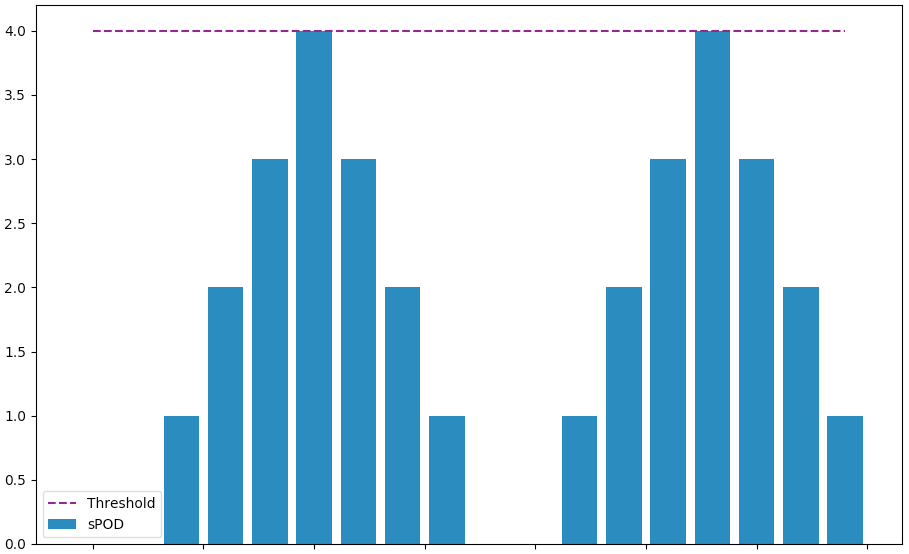
\includegraphics[width=0.7\textwidth]{highThreshold}
	\caption[Umbral elevado.]{Con un umbral muy elevado, puede darse el caso de que todo sean valles hasta estar demasiado cerca del obstáculo.}\label{fig:highThreshold}
\end{figure}

Por el contrario, si el umbral es muy bajo, ver figura \ref{fig:lowThreshold}, hará que los valles candidatos se vean reducidos, haciendo que el drone no pueda pasar por espacios estrechos.
 \begin{figure}[H]
	\centering
	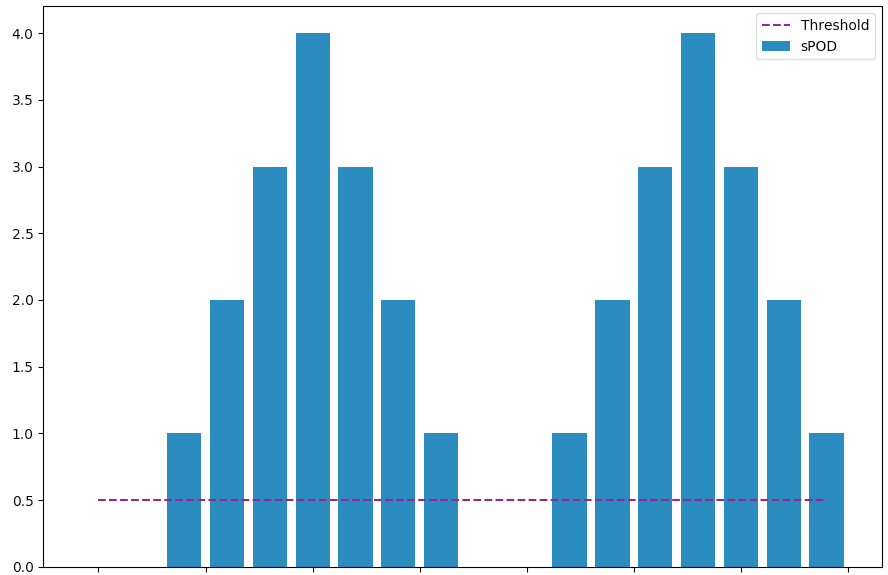
\includegraphics[width=0.7\textwidth]{lowThreshold}
	\caption[Umbral bajo.]{Con un umbral muy bajo, puede darse el caso de que los valles sean muy estrechos, o incluso inexistentes}\label{fig:lowThreshold}
\end{figure}



\section{Dispositivos Físicos}

\subsection{Raspberry Pi}

\begin{table}[H]
	\begin{center}
		\rowcolors {2}{gray!35}{}
		\begin{tabular}{l | c}\hline
			\toprule
			Componente & Raspberry Pi 3B\\
			\otoprule
			CPU & BCM2837\\
			Núcleos & 4\\
			Velocidad & 1.2GHz\\
			RAM & 1GB\\
			Coms & Ethernet, WiFi, Bluetooth\\
			USB & 4 (2.0)\\
			GPIO & 40\\
			Consumo máximo & 6.7W\\
			\bottomrule
		\end{tabular}
		\caption{Componentes de una Raspberry Pi 3 Model B}
		\label{tb:raspi3hardware}
	\end{center}
\end{table}

\noindent Una Raspberry Pi es un pequeño ordenador desarrollado en UK por la Raspberry Pi Foundation, con la intención de promover el aprendizaje de informática básica en colegios y países en desarrollo. El modelo base se compone de una única placa de medidas 85mm x 56mm (LxA), y unos 42g de peso.\\Concretamente el modelo empleado es una Raspberry Pi 3B, y consta de los componentes detallados en la tabla \ref{tb:raspi3hardware}



\noindent Su reducido tamaño y bajo consumo lo hacen ideal para este tipo de proyecto. \\En este caso se utiliza bajo una distribución GNU/Linux llamada Raspbian\footnote{Descargable desde: https://www.raspberrypi.org/downloads/raspbian}, basada en Debian. Para tratar de mejorar su rendimiento y reducir al mínimo el consumo, se ha escogido la versión Lite del sistema, es decir, un sistema mínimo sin entorno de escritorio y con la mayor parte de servicios desactivados por defecto.

\begin{figure}
	\centering
	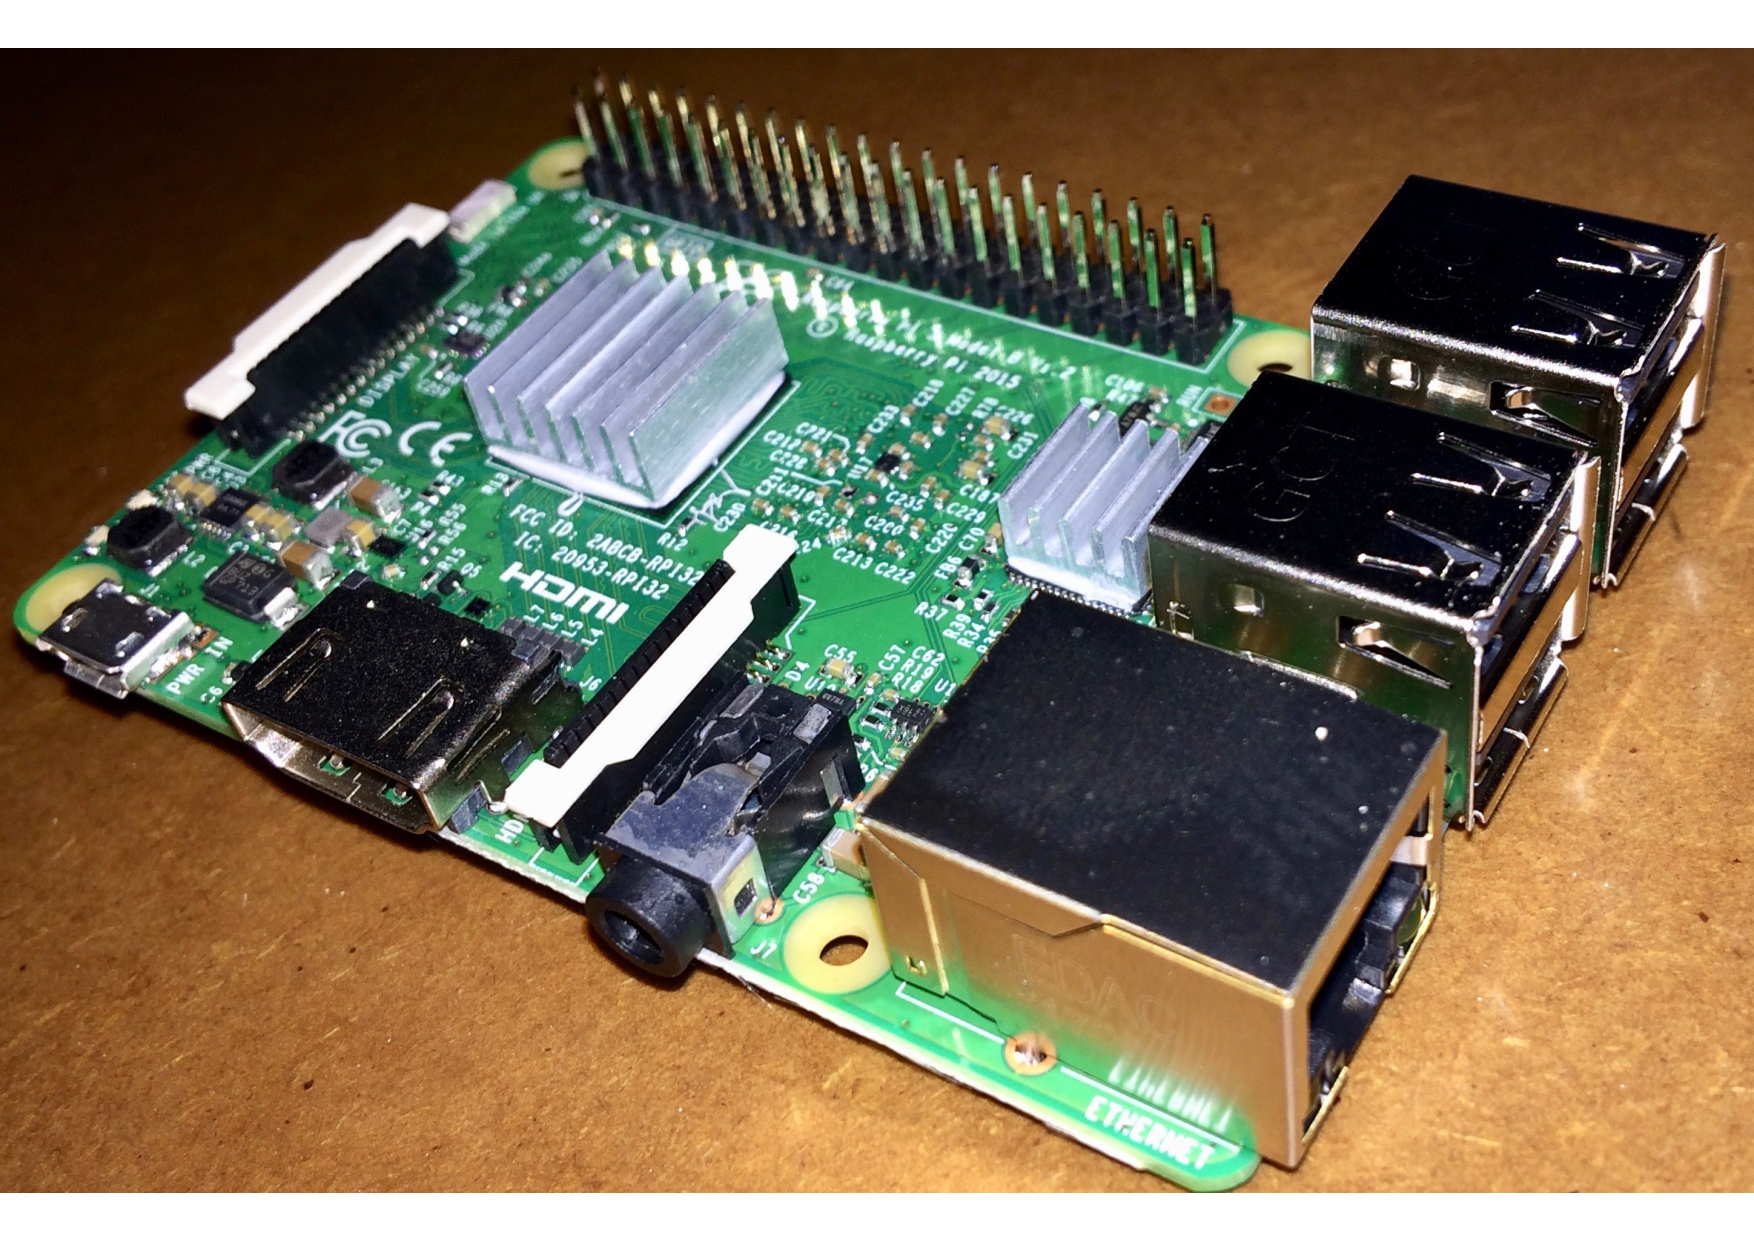
\includegraphics[width=0.9\textwidth]{raspi}
	\caption{Raspberry Pi 3.}\label{fig:raspi3b}
\end{figure}

Una vez descargado el sistema, este ha sido instalado en una micro SD mediante el siguiente procedimiento por consola\footnote{Realizado en OSX, aunque en Linux es muy similar}:
\begin{itemize}
\item\code{diskutil list} Permite localizar el dispositivo en el que se encuentra la tarjeta. En nuestro caso \code{/dev/disk4}
\item\code{diskutil umountDisk /dev/disk4} Permite desmontar el volumen. 
\item\code{sudo dd if=raspbian-stretch.img of=/dev/rdisk4 bs=1m} El comando \code{dd} copia la entrada estándar a la salida estándar. Mediante \code{if/of} se establece el fichero de entrada/salida. Mediante \code{bs} se establece el tamaño de bloque a copiar. Se está utilizando \code{/dev/\underline{\textbf{r}}disk4} en lugar de \code{/dev/disk4} debido a la capacidad de OSX de trabajar con dispositivos en bruto, \textit{raw}, de forma que es posible acceder al dispositivo de forma directa\footnote{Véase \code{man hdiutil}, sección \textit{DEVICE SPECIAL FILES}}, sin almacenar en un buffer la lectura del archivo, proporcionando velocidades de escritura/lectura hasta 20 veces más rápidas.
\end{itemize}


Una vez realizados estos pasos, se puede insertar la microSD en la Raspberry Pi. Para encenderla basta con utilizar el puerto micro-usb de que dispone.\\La Raspberry Pi 3 requiere de una fuente de alimentación capaz de proporcionar 2,5A\footnote{Véase https://www.raspberrypi.org/help/faqs/\#power} para funcionar al máximo nivel de estrés para el procesador y alimentar dispositivos USB.

Sin embargo, este no es estrictamente nuestro caso, véase la subsección \ref{subsubsec:Modificaciones}. Se requiere un dispositivo cuyo consumo sea lo más reducido posible, pero que sea rápido en la ejecución, y que muestre poca latencia en operaciones de \code{IO}, que es donde se encuentra el cuello de botella.

Una vez encendida, se accede a ella con el usuario por defecto \code{pi} y la contraseña por defecto \code{raspberry}. Obviamente ambas \textbf{han sido cambiadas} por motivos de seguridad.



\subsubsection{Modificaciones}
\label{subsubsec:Modificaciones}

\begin{figure}
	\centering
	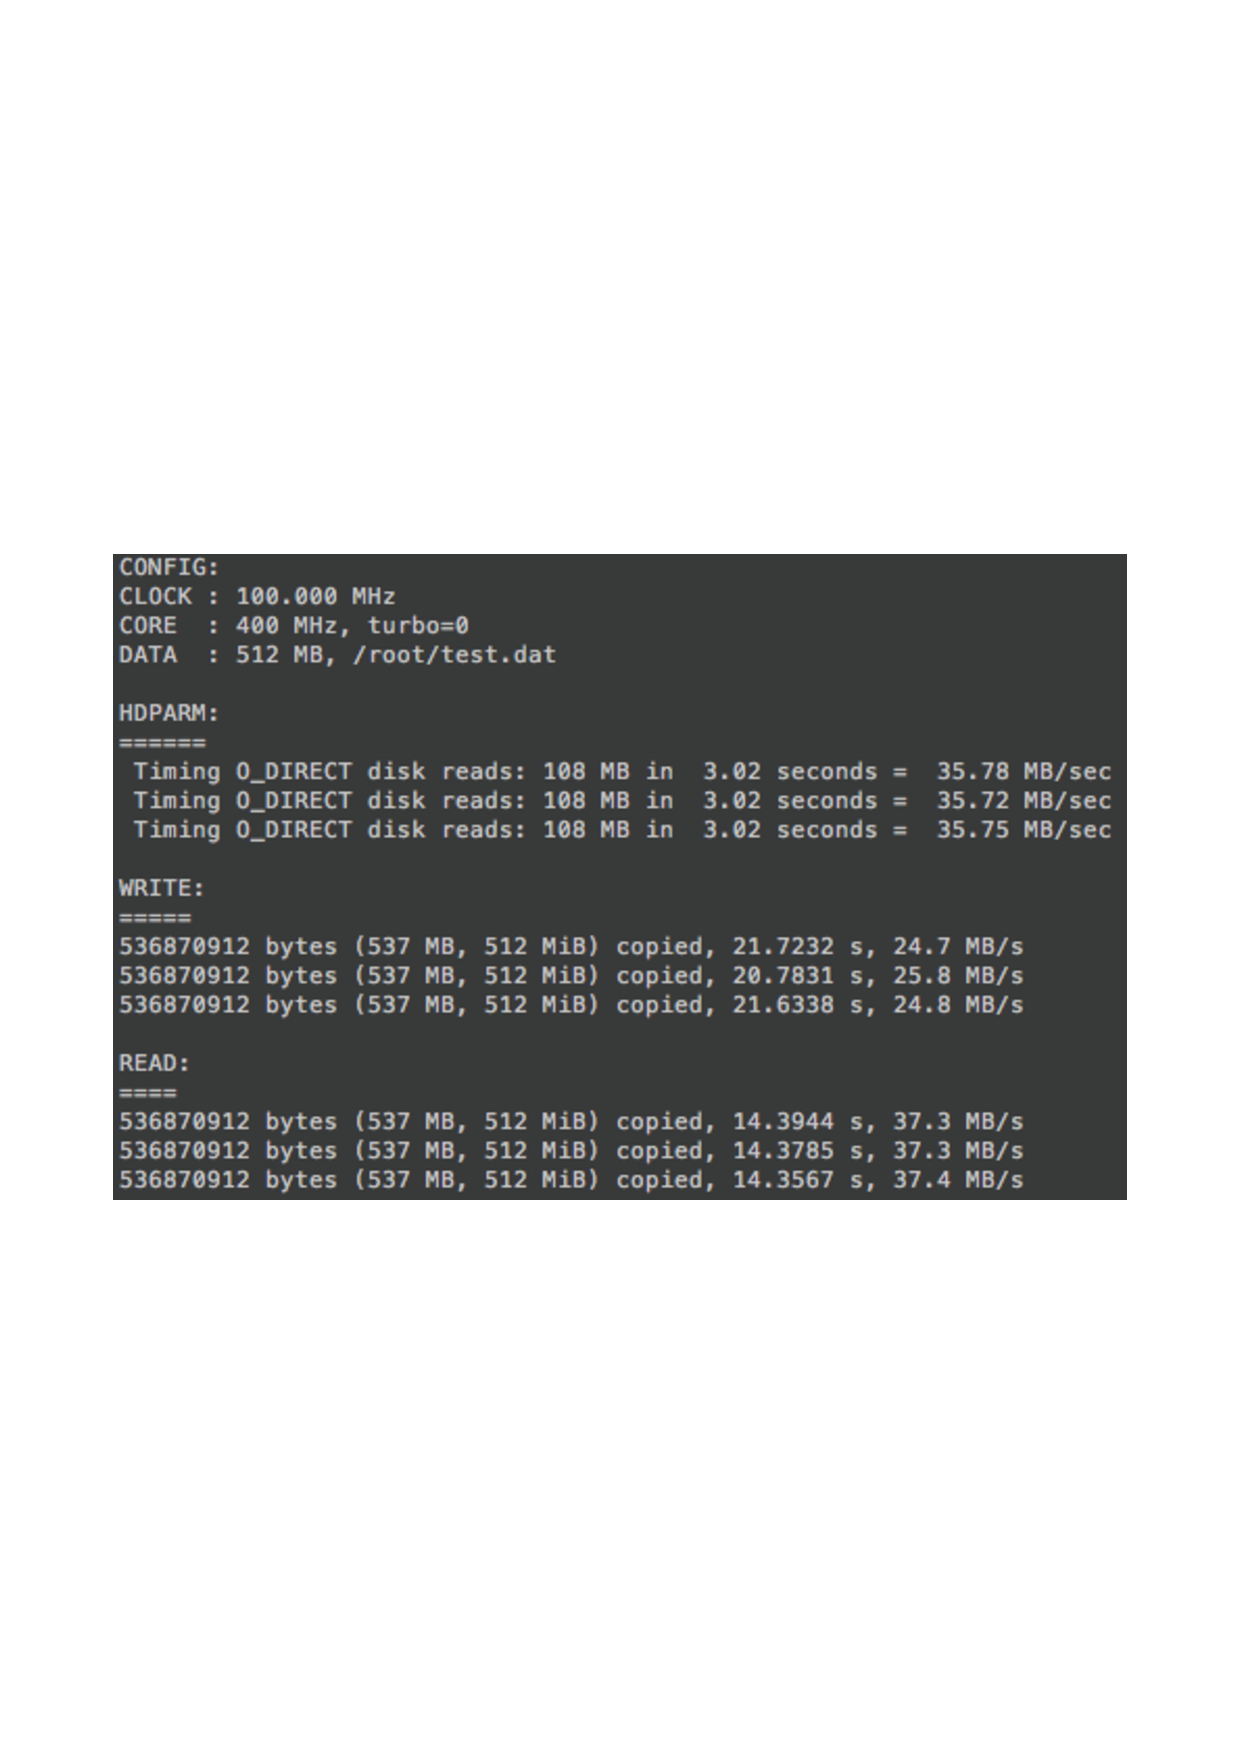
\includegraphics[width=0.9\textwidth]{sdbench}
	\caption{Benchmark de lector microSD OC.}\label{fig:sdbenchmark}
\end{figure}

\begin{itemize}
\item Se ha desactivado el puerto HDMI para reducir el consumo en \textasciitilde{}30mA: \\Para ello se ha incluido en \code{/etc/rc.local} la línea \code{/usr/bin/tvservice -o}. Descrito en \citep{wiki:PowerSaving}.
\item Se ha overclockeado el lector de microSD a 100MHz, en lugar de los 50MHz por defecto: \\Para ello se ha incluido en \code{/boot/config.txt} la línea \code{dtparam=sd\_overclock=100}.\\Y que arroja los resultados mostrados en la figura \ref{fig:sdbenchmark}. Descrito en \citep{wiki:OCSD} y \citep{wiki:OCSDWifiFix}.
\item Se han incluido una serie de disipadores para evitar sobrecalentamiento de la placa. Así como un pequeño ventilador de bajo consumo.
\end{itemize} 


\subsection{Controladora de Vuelo}

Una controladora de vuelo (\textit{FC} de aquí en adelante) es un pequeño circuito integrado, que contiene un procesador, una serie de sensores, y una serie de entradas y salidas. 
\begin{figure}
\centering
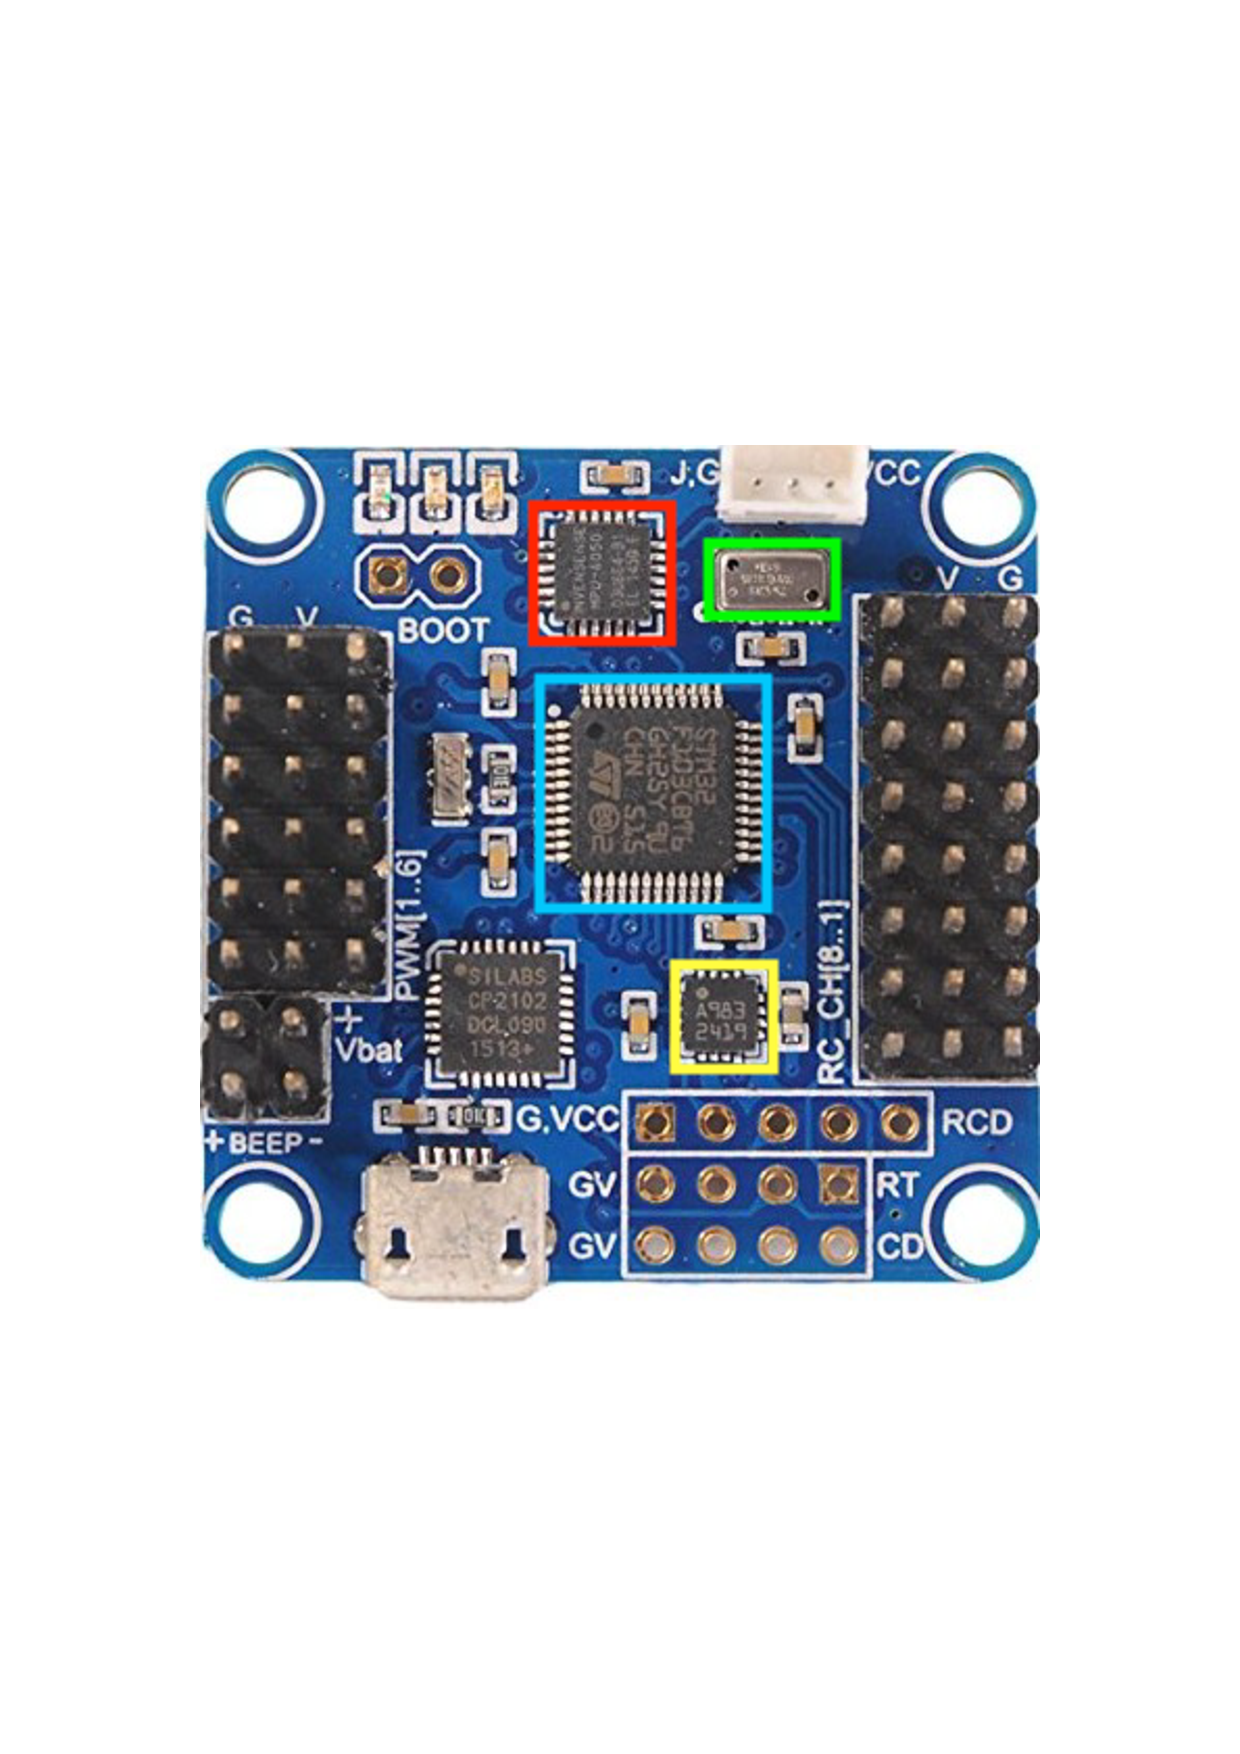
\includegraphics[width=0.5\textwidth]{flip32}
\caption{Controladora de Vuelo Flip32.}\label{fig:fc}
\end{figure}
La FC se encarga de mantener el sistema de estabilización del drone, tomando medidas de los sensores de que dispone, tales como un acelerómetro, giroscopio, magnetómetro, barómetro... etc. 

En el caso de la FC usada para este proyecto, llamada Flip32 y mostrada en la figura  \ref{fig:fc}, se dispone de un IC MPU-6050, en rojo, con acelerómetro y giroscopio, así como de un barómetro M55611, en verde, y un magnetómetro HMC5883L, en amarillo.
El núcleo de esta pequeña placa es un procesador STM32F103, en cyan, a 72MHz y basado en arquitectura ARM el cual dispone de dos puertos serie, que permiten establecer comunicación entre la FC y otros dispositivos, como emisoras u otros sensores.

El puerto micro-USB de que dispone es utilizado para establecer comunicación entre el configurador de opciones del drone, o en el caso de nuestro proyecto, para hacer uso del \hyperref[subsec:MSP]{MultiWii Serial Protocol}. 


\subsubsection{Entradas}
En el lado derecho de la figura \ref{fig:fc} pueden verse una serie de pines que actúan como 8 canales de entrada desde el receptor de radio.
Dichos canales de entrada, por defecto, reciben una señal modulada en ancho de pulso o \hyperref[subsec:PWM]{PWM}

 

\subsubsection{Salidas}
En el lado izquierdo de la figura \ref{fig:fc}, pueden verse otros pines que actúan como salida de señal hacia los controladores de velocidad de los motores del drone (ESC o \textit{Electronic Speed Controller}).
Estos pines de salida, emiten una señal que será interpretada por los ESC del drone, para determinar la frecuencia dada al voltaje que alimenta los motores. En el caso de nuestro proyecto, los ESC disponibles reciben una señal PWM.

\newpage
\subsubsection{Sensores}
\label{subsubsec:sensors}
La controladora de vuelo Flip32 en su versión más completa, dispone de los siguientes sensores:
\begin{itemize}
\item IMU\footnote{Unidad de Medición Inercial.} MPU-6050: Se trata de un circuito integrado compuesto de un acelerómetro de tres (3) ejes y un giroscopio de tres (3) ejes. El acelerómetro mide las fuerzas en los tres diferentes ejes (en \textit{g}) , el giroscopio se encarga de medir la velocidad angular en cada uno de los tres ejes (en degº/s )
\item Magnetómetro HMC5883L: Se trata de un pequeño magnetómetro digital capaz de medir el campo magnético terrestre (en Gauss). Se debe tener en cuenta que según la posición en el planeta, el campo magnético varía entre \si{\gauss{0.25}} - \si{\gauss{0.65}}, así como la declinación magnética de la zona en la que se realiza la medición.\footnote{Disponible en: http://magnetic-declination.com/}
\item Barómetro M55611: Se trata de un altímetro de alta precisión, con resoluciones de hasta 10cm, que funciona midiendo la presión atmosférica (en milibar). Hay que tener en cuenta que los cambios de presión, como los generados por las hélices del drone, hacen variar la medida del sensor. Por ello, en el caso de usarlo, se cubre con un pequeño filtro de un material absorbente, lo suficientemente denso como para evitar el contacto directo entre una corriente de aire y el sensor.
\end{itemize}

\subsection{Sensores de distancia}
\label{subsec:hcsr04}
Para medir la distancia existente entre los diferentes obstáculos y el agente, se ha hecho uso de sensores de ultrasonidos. Estos sensores, habitualmente llamados \emph{sonar}, envían un pulso de ultrasonidos en la dirección en que apuntan, y reciben el eco de dicho pulso. Una vez recibido el eco, es posible determinar el tiempo que ha tardado en recorrer el espacio, sabiendo la velocidad del sonido en condiciones ideales, es posible conocer la distancia aproximada del objeto. 
La ecuación \ref{eq:dstSound} refleja este cálculo.
\begin{equation}
\label{eq:dstSound}
e = \frac{2*v}{t}
\end{equation}
Donde $e$ es el espacio recorrido, $v$ es la velocidad del sonido, se suele tomar $340m/s$, y $t$ es el tiempo transcurrido entre el envío del pulso y la recepción del eco. Se multiplica por $2$ dado que el sonido tiene que ir y volver.

Los sensores utilizados, tienen como nomenclatura HC-SR04 \citep{wiki:sparkHCsr04}, y son muy conocidos por dar resultados relativamente buenos, y por su asequibilidad. 
Son capaces de obtener medidas de entre 400 cm y 2 cm con una precisión de $\pm$5 mm, pero para no forzar los extremos en este proyecto se ha establecido una distancia máxima de 350 cm y una mínima de 10 cm. 

Disponen de una interfaz muy sencilla. Se trata únicamente de cuatro pines que deben ser conectados, uno de alimentación, uno de tierra, uno para disparar el pulso y uno para la recepción del eco. 

En la figura \ref{fig:sr04} pueden verse los pines y los elementos de disparo y recepción del ultrasonido. 

\begin{figure}[H]
	\centering
	\includegraphics[width=0.9\textwidth]{sr04}
	\caption[Sensor HC-SR04]{Sensor HC-SR04. Detalle de los pines y cabezales de envío y recepción de ultrasonido}\label{fig:sr04}
\end{figure}

\subsubsection{Desventajas}
El uso de ultrasonidos para detectar objetos y distancias presenta una serie de inconvenientes que serán detallados en mayor profundidad en el capítulo \ref{cap:RelvAsp}. Por enunciar algunos, 
\begin{itemize}
\item La velocidad del desplazamiento del sonido por el medio cambia con la temperatura. No es una variación muy grande, pero impide una precisión grande por parte de estos sensores.
\item Los sensores de ultrasonidos son susceptibles a ecos provenientes de otros sensores, lo que dificulta mucho la posibilidad de disparar varios al mismo tiempo.
\item El sonido puede verse absorbido por un obstáculo hecho de un material absorbente, falseando las medidas del sensor.
\item El sensor tiene un rango de acción de 30º, lo cual dificulta su posicionamiento y detección de obstáculos de forma precisa, es decir, es fácil conocer la distancia a que se encuentra un obstáculo, pero no saber en que posición del arco de 30º se encuentra exactamente.
\item Este sensor funciona a 5V, y la RaspberryPi a 3.3V, con lo que debe crearse un mecanismo para reducir este voltaje para no dañar los pines del procesador de la Raspberry.
\end{itemize}

\newpage





\section{Protocolos}

\subsection{Pulse Width Modulation}\footnote{PWM no es un protocolo como tal, sino una técnica de codificación de la información haciendo uso de una señal analógica. Se ha incluido en esta sección por simplicidad.}
\label{subsec:PWM}

La modulación por ancho de pulso \citep{wiki:PWM}, se basa en medir el transcurso de tiempo entre el flanco de subida de una señal, y el flanco de bajada, tal y como puede verse en la figura \ref{fig:PWM}.
En este contexto, un receptor de radio recibe una señal de la emisora,  y genera una señal PWM acorde que será transmitida a la FC.
Estas son capaces de entender señales de entre 1000 y 2000\si{\us}. Cualquier valor por debajo, o por encima, haría entrar la controladora en FailSafe\footnote{Al recibir una señal inválida por parte del receptor, la controladora de vuelo puede ser configurada para desactivar el drone, mantener la última medida buena conocida, intentar aterrizar... etc. Este modo es conocido como FailSafe}. 
En el caso de este proyecto, se ha determinado que no se hará uso de este método para la comunicación entre la Raspberry Pi y la controladora de vuelo, véase la subsección \ref{subsec:MSP}, y por lo tanto el uso de estos pines queda descartado.

Sin embargo, la comunicación entre la FC y los ESC se realiza mediante este tipo de señal, por ello se ha considerado relevante explicar, brevemente, su funcionamiento.
\begin{figure}[H]
	\centering
	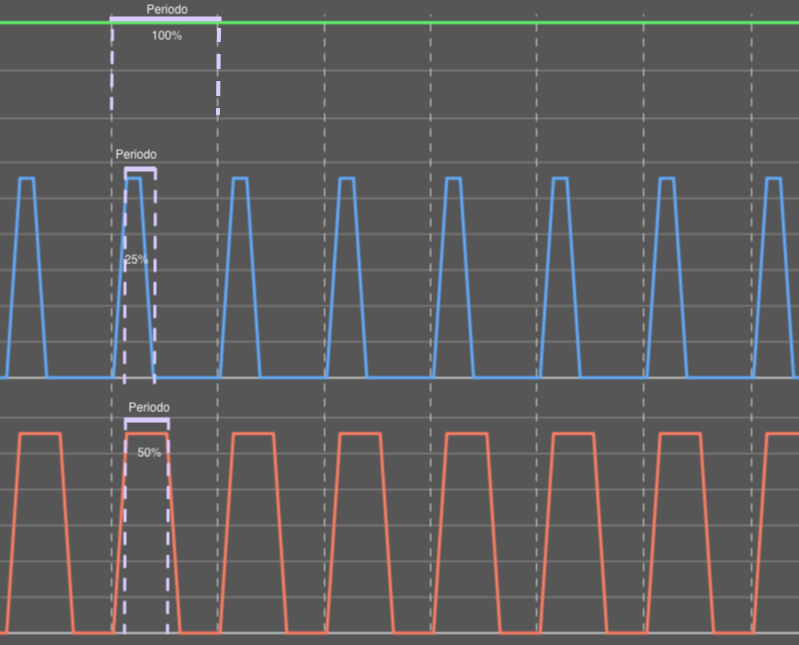
\includegraphics[width=0.9\textwidth]{PWM}
	\caption[PWM. Modulación en Ancho de Pulso.]{Modulación en Ancho de Pulso. Arriba 100\% del ciclo usado. Centro 25\% del ciclo usado. Abajo 50\% del ciclo usado}\label{fig:PWM}
\end{figure}


\subsection{MultiWii Serial Protocol}
\label{subsec:MSP}

MultiWii es un software de control de multirotores y está basado en componentes de la Nintendo Wii. Concretamente, los mandos de control de la consola de Nintendo poseen tres acelerómetros para determinar la posición angular y medir aceleraciones laterales. El problema es que los acelerómetros no son precisos para variaciones pequeñas, de forma que Nintendo creó un complemento que se podía conectar al propio mando, el Wii Motion Plus, que dispone de tres giroscopios, de forma que unidos a los tres acelerómetros iniciales, proporcionan una medición mucho más precisa de la posición del mando.

A los primeros creadores del sistema de control MultiWii se les ocurrió la posiblidad de hacer uso de estos sensores para crear un sistema de control de drones, \citep{wiki:MultiWiiHistory}. Uniendo estos sensores a un controlador, en principio se trató de un Arduino Mini, y programándolo para tal efecto, se logra crear una FC algo rudimentaria, pero que da muy buenos resultados.

Para crear un entorno amigable para el usuario común, se desarrolló una aplicación de escritorio capaz de configurar los parámetros de esta controladora de vuelo poco convencional. De alguna forma debía lograrse una comunicación entre la FC y la aplicación, y así se implementó MultiWii Serial Protocol, \citep{wiki:MSPDefinition}.\\Conocido como \textit{MSP}, se trata de un protocolo que se ha mantenido en diferentes implementaciones de sistemas de control de vuelo. No solo aquellos basados en sensores de la Nintendo Wii controlados por Arduino, sino en otros más modernos y potentes que han ido surgiendo los últimos años. Como el utilizado en nuestro proyecto.
\newpage
Es un protocolo eficiente y sencillo, que permite una comunicación rápida y completa. Su composición puede verse en la figura \ref{fig:MSPlayout}
\begin{figure}[H]
	\centering
	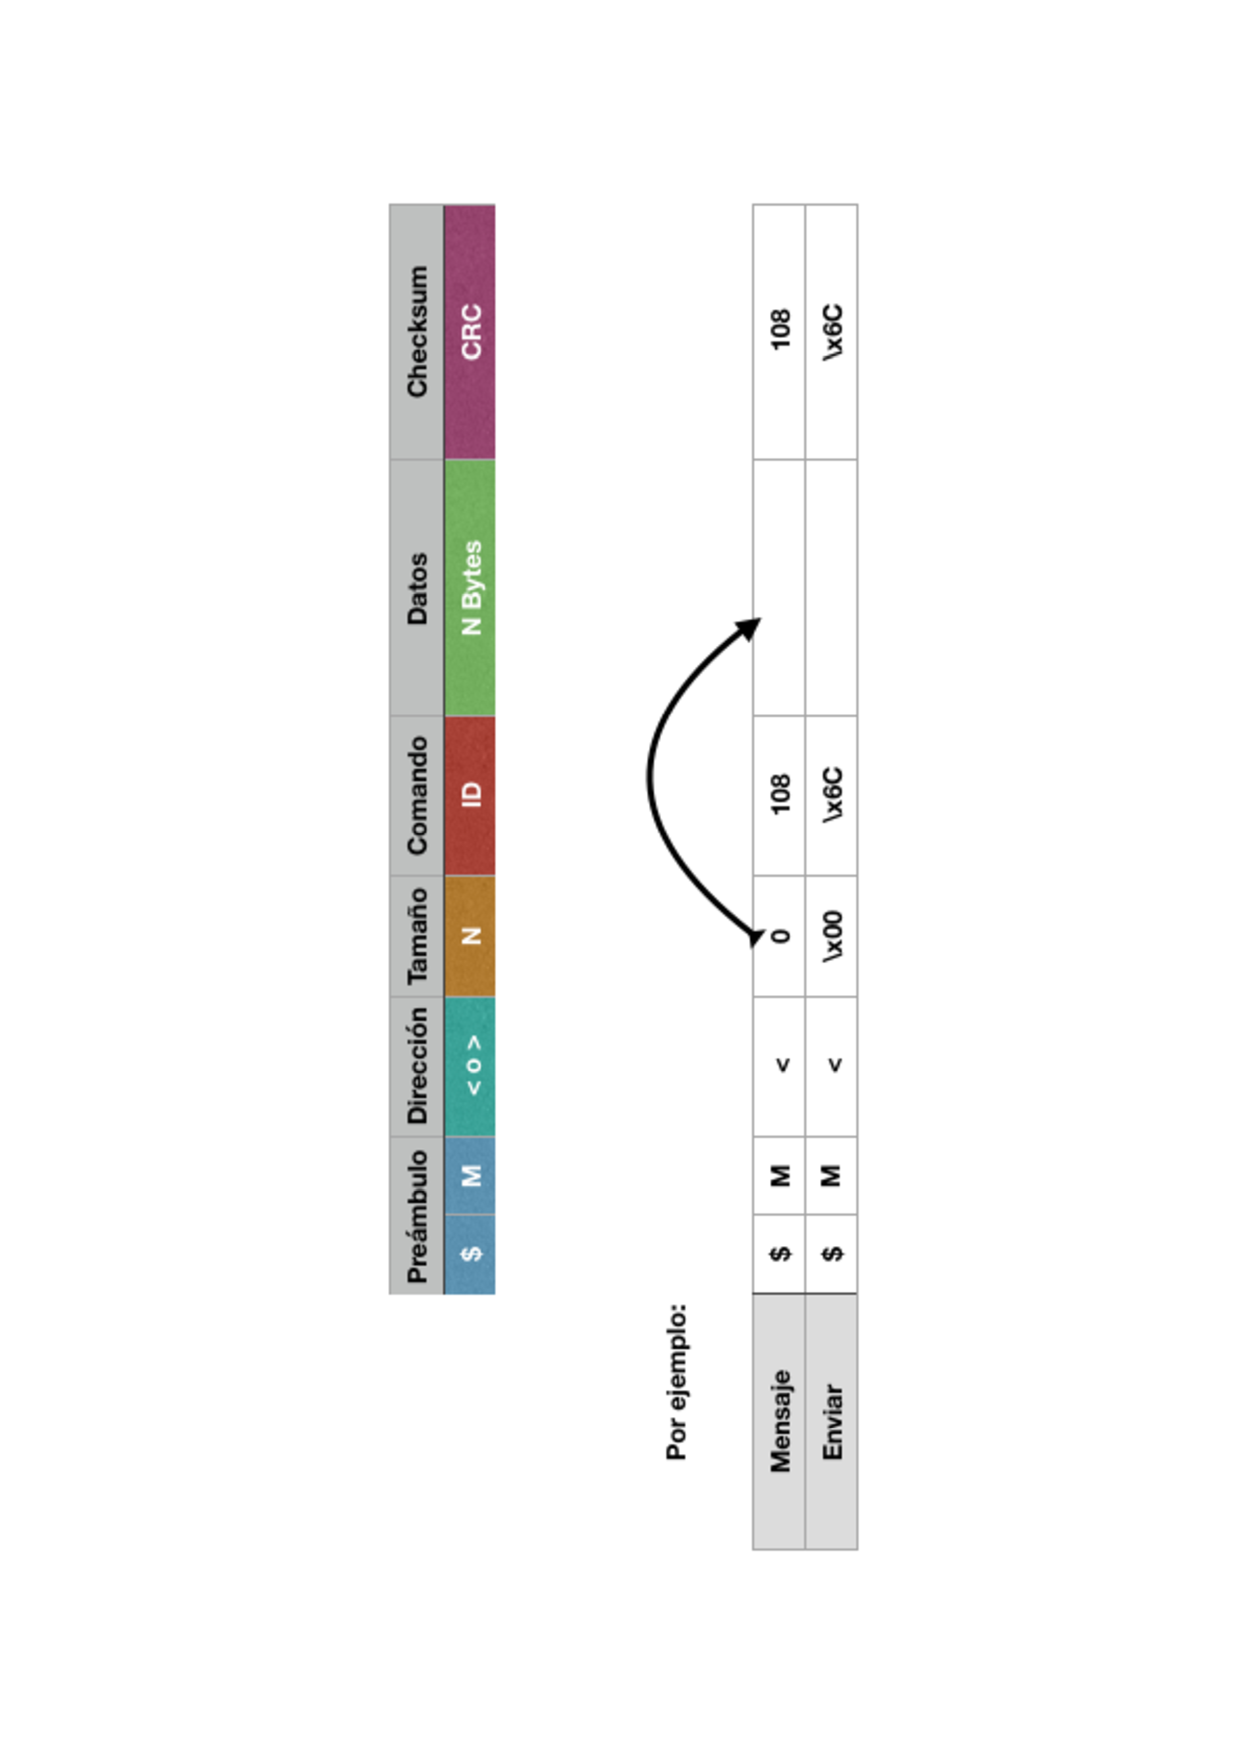
\includegraphics[width=0.9\textwidth]{MSPlayout}
	\caption{Composición de un mensaje MSP.}\label{fig:MSPlayout}
\end{figure}

\begin{itemize}
\item Preámbulo: Se trata de dos caracteres ASCII que determinan el comienzo de un nuevo mensaje. Se compone de un símbolo `\$' y una letra `M'.
\item Dirección: Se trata de un caracter ASCII que determina la dirección del mensaje, \textbf{hacia} la controladora `<' o \textbf{desde} la controladora `>'.
\item Tamaño: Se trata de un byte que determina el tamaño, en bytes, de los datos enviados o recibidos.
\item Comando: Se trata de un byte que determina el comando a ejecutar. Véase la tabla  \ref{tb:MSP_MESSAGES} para una relación de los comandos implementados.
\item Datos: Se trata de una serie de bytes, de longitud definida por el byte <\textit{tamaño}>, que establecen el resto de parámetros a pasar con la función definida por el byte <\textit{comando}>.
\item Checksum: Se trata de un byte de control. Se define su valor mediante la función XOR entre <\textit{tamaño}>, <\textit{comando}> y cada byte contenido en <\textit{datos}>


\end{itemize}

En el caso de nuestro proyecto, se hará uso de este protocolo dado que existe la posibilidad de establecer la recepción de los canales de radio a través de un puerto serie, así como de solicitar información sobre el estado del drone a la FC. Es decir, en lugar de utilizar un receptor de radio, se utilizará un puerto serie para obtener la telemetría\footnote{Se define telemetría como un sistema de medición de magnitudes a distancia; en este contexto el término se ha desvirtuado y se entiende como la información que es transmitida de vuelta a la emisora de vuelo, siendo esta generalmente información de los sensores de la FC, GPS o voltaje disponible en la batería.}, y establecer las entradas de los canales de radio. 
En la tabla \ref{tb:MSP_MESSAGES} se dispone de los mensajes implementados para la realización de este proyecto. 


\afterpage{
\clearpage
\begin{landscape}
\begin{table}[H]
	\begin{center}	
		\rowcolors {2}{gray!35}{}
		\begin{tabular}{m{5cm} | c | m{4cm} | c | m{7cm}}\hline
			\toprule
			Mensaje & Código & Estructura & Parse & Descripción\\
			\otoprule
			MSP\_MOTOR & 104 & 8x UINT16 & <8H & Devuelve la señal PWM que los ESC envían a los motores.\\
			MSP\_RC & 105 & 18x UINT16 & <18H & Devuelve la señal PWM disponible en cada canal.\\
			MSP\_ATTITUDE & 108  & 3x INT16 & <3h & Devuelve las inclinaciones de los ejes X e Y, así como la orientación.\\
			MSP\_ANALOG & 110 & 1x UINT8 3x UINT16 & <B3H & Devuelve el estado de los sensores incluidos en la FC: voltaje de la batería, RSSI, corriente instantánea y consumo\\
			MSP\_SET\_RAW\_RC & 200 & Nx UINT16 & N/A & Establece el valor de los canales de radio-control.\\
			MSP\_SET\_RAW\_MOTOR & 214 & Nx UINT16 & N/A & Establece la señal PWM a enviar a los motores.\\
			\bottomrule
		\end{tabular}
		\caption{Mensajes MSP. Estructura de datos y representación}
		\label{tb:MSP_MESSAGES}
	\end{center}
\end{table} 

La columna \textit{Mensaje} sigue esta nomenclatura por razones históricas, para mantener cierta coherencia con la tabla disponible en la descripción del protocolo MultiWii \citep{wiki:MSPDefinition}. La columna \textit{Código} establece el número de comando enviado. Los comandos que empiezan por 1, se corresponden con solicitudes de información, y aquellos que comienzan por 2 son órdenes. Este valor será utilizado por la FC para establecer el parseo de la información enviada, de ser alguna. La columna \textit{Estructura} establece el tipo y la cantidad de cada dato que se envía o recibe. La columna \textit{Parse} establece el tipo de parser que se aplicará a la respuesta recibida de la FC. Nótese que solo se define el parser para los comandos que comienzan por 1, es decir, para las solicitudes de información.
\end{landscape}
\clearpage
}
La información del parser proporciona la manera de decodificar la cadena de bytes devuelta por la FC al realizlar una solicitud. Para ello se ha seguido la nomenclatura utilizada en el módulo \textit{struct} de Python 3.5 \citep{wiki:PythonStruct}, y  descrita en la tabla \ref{tb:PY35STRUCT}

\begin{table}[H]
	\begin{center}	
		\rowcolors {2}{gray!35}{}
		\begin{tabular}{c | p{10cm}}\hline
			\toprule
			Elemento & Descripción\\
			\otoprule
			`<', `>' & Little o Big Endian respectivamente. Establece la ubicación del byte menos significativo, y por lo tanto determina la dirección de lectura de los grupos de bytes de la cadena recibida.\\
			`B' & Carácter utilizado para representar un entero de un byte sin signo.\\
			`H' & Carácter utilizado para representar un entero de dos bytes sin signo.\\
			`c' & Carácter utilizado para representar un carácter de un byte.\\
			\bottomrule
		\end{tabular}
		\caption{Nomenclatura del módulo Struct de la implementación 3.5 de Python}
		\label{tb:PY35STRUCT}
	\end{center}
\end{table} 

Los enteros sin signo representados en la tabla \ref{tb:PY35STRUCT}, tienen su equivalencia a enteros con signo mediante el mismo carácter en minúscula.\\La implementación realizada sigue un paradigma funcional, de forma que la función utilizada para leer las respuestas de la FC puede ser utilizada con nuevas solicitudes de información, con tan solo pasar un nuevo parser en forma de cadena de texto.



\subsection{Secure SHell}
\label{subsec:ssh}
Secure SHell o \textit{SSH} \citep{wiki:SSH} de aquí en adelante, es un protocolo de red cifrado el cual se basa en el uso de claves públicas compartidas para crear un canal de comunicación seguro en una red no segura. Al aceptar una conexión, el servicio SSH presenta una shell sobre la que el cliente puede realizar las operaciones necesarias y propias de su nivel de privilegio. Además proporciona la posibilidad de redirigir el sistema de ventanas remoto al cliente, aunque en este caso se está haciendo uso de una versión reducida del SO, y por lo tanto no presenta entorno de escritorio. El acceso a la Raspberry Pi que controla el drone, se lleva a cabo mediante el uso de este protocolo, siguiendo los siguientes pasos para su configuración:
\begin{itemize}
\item Generar el par de claves pública-privada en el cliente mediante el comando \code{ssh-keygen}
\item Copiar la clave pública del cliente en el archivo \code{.ssh/authorized\_keys} de la carpeta \code{home} del usuario a utilizar en el sistema remoto.
\item Editar el archivo \code{/etc/ssh/sshd\_config} para:
	\begin{itemize}
	\item permitir unicamente acceso a usuarios que envíen una clave pública contenida en \code{authorized\_keys}.
	\item desactivar el acceso al usuario root, estableciendo la propiedad \code{PermitRootLogin} a \code{no}.
	\item desactivar el acceso por contraseña, estsableciendo la propiedad \code{PasswordAuthentication} a \code{no}.
	\end{itemize}	 
\end{itemize} 

De esta forma se logra dotar de acceso seguro a un cliente autorizado. Al tratar de conectar al sistema de control del drone, se muestra un banner en el que se advierte a usarios malintencionados de la existencia de un log de conexiones recibidas. 
Para tratra de mitigar ciertos intentos de intrusión en el sistema, algo tan simple como cambiar el puerto en el que responde el servidor SSH, se ha mostrado tremnedamente efectivo contra los ataques automatizados más simples y comunes.

\subsection{WebSocket}
\label{subsec:WebSocket}
Se trata de un protocolo de comunicaciones full-duplex sobre una conexión TCP. Fueron estandarizados por el IETF como RFC 6455, \citep{wiki:WebSocket6455, wiki:WebSocketWiki}, en el año 2011.  

La comunicación se realiza a través del puerto 80 identificando el recurso como \textit{ws}, o del 443 si se utiliza una conexión cifrada  identificando el recurso como \textit{ws\textbf{s}}, y es actualmente implementado por la mayoría de los navegadores. 

En el caso de este proyecto se utilizarán WebSockets para realizar el proceso de \textit{signaling} hacia el servidor WebRTC, ver subsección \ref{subsec:WebRTC}, que se estará ejecutando en la RaspberryPi, para que este inicie la transmisión de vídeo en tiempo real y así poder visualizarlo. Dicha conexión será cifrada mediante SSL/TLS haciendo uso del certificado generado y firmado por una CA\footnote{Certificate Authority. Una entidad que proporciona certificados digitales.} de confianza.

Mediante WebSockets se establecerá el mecanismo para coordinar la comunicación y enviar mensajes de control al servidor de vídeo en tiempo real. Este proceso, denominado \textit{signaling}, comporta tres tipos de información:
\begin{itemize}
\item Session Control Messages: Mensajes de Control de Sesión. Utilizados para iniciar o finalizar la comunicación, así como para reportar errores.
\item Network Configuration: Configuración de Red. Utilizados para enviar la dirección IP y puerto de comunicación desde el cliente hacia el servidor.
\item Media Capabilities: Capacidades de los dispositivos de Medios. Utilizados para establecer el tipo de codec, resolución, bitrate... etc.
\end{itemize}

Este intercambio de información deberá completarse de forma correcta antes de comenzar la transmisión entre el cliente y el servidor. 


\subsection{WebRTC}
\label{subsec:WebRTC}
Se trata de un proyecto de código abierto que proporciona comunicación en tiempo real mediante una API, para facilitar el intercambio de información entre pares, idealmente, aunque puede darse el caso de requerir el paso de esta información por un tercer servidor. Esta iniciativa involucra a Google, Mozilla y Opera entre otros, \citep{wiki:WebRTCorg, wiki:WebRTCmdn}.

Se apoya en ICE o Interactive Connectivity Establishment, \citep{wiki:ICE} un framework utilizado para lograr que dos clientes se comuniquen entre sí, sin necesidad de un servidor intermedio que haga de negociador y de esta forma conseguir que la comunicación sea lo más ágil y rápida posible. Para lograrlo, pese al enmascaramiento de los clientes tras múltiples NAT\footnote{Network Address Translation. Con la masificación de internet se ha llegado a un punto en el que el protocolo IPv4 no dispone de más espacio de direccionamiento, es decir, no quedan direcciones IPv4. En lugar de migrar los diferentes elementos de una arquitectura de red (como switches, routers, servidores y demás) al protocolo de internet IPv6, que proporciona un espacio de direccionamiento \emph{mucho} mayor ($2^{128}$ direcciones), los proveedores de servicios de internet, crean redes de redes usando como \textit{recepcionista} el NAT. Lo cual dificulta \emph{terriblemente} el encaminamiento de información entre pares. Sobre todo cuando crean NATs de dispositivos que usan NATs}, hace uso de:
\begin{itemize}
 \item Servidores STUN (Session Traversal Utilities for NAT), que se encuentran en el lado público de esta. Permiten detectar el uso de NAT, y encuentran el mapeo de IP y puerto realizado para la aplicación del cliente. De esta forma un cliente tras una NAT es capaz de conocer su IP pública y el puerto que utiliza para \textit{salir} a internet, \citep{wiki:STUN}.
 \item Servidores TURN (Traversal Using Relays around NAT), como último recurso. En el caso de que no se pueda realizar la comunicación P2P, el sistema pasa a utilizar un servidor que hace de repetidor, lo cual obviamente añade cierto retardo y supone una gran carga para estos. El protocolo TURN se encarga de proporcionar IP y puerto para obtener una conexión con estos servidores \textit{repetidores} o \textit{retransmisores}, \citep{wiki:TURN}.
\end{itemize}


El funcionamiento general de una comunicación entre pares (Alice y Bob, por supuesto) haciendo uso de la API WebRTC es como sigue: 
\begin{itemize}
\item[1] Alice y Bob establecen comunicación haciendo uso del ICE, el cual trata de comunicarlos por un canal directo, con la menor latencia posible haciendo uso del protocolo UDP. Para ello es necesario utilizar servidores STUN. Google provee de un par de servidores STUN de uso libre. Si la comunicación por UDP falla, ICE trata de establecerla bajo TCP (primero HTTP y despues HTTPS). Si la comunicación directa falla (generalmente debido a NAT transversales o firewalls), ICE hará uso de servidores TURN que harán de repetidores de los mensajes del cliente.
\item[2] Signaling. La aplicación negocia el tipo de comunicación que espera, es decir, el codec de video, la resolución, el codec de audio, bitrate... etc. Y establece los orígenes de vídeo/audio para ambos peers. En la documentación de WebRTC no se define la forma en que se debe transmitir la información, de manera que en este proyecto se ha escogido hacerlo a través de WebSockets, ver la subsección \ref{subsec:WebSocket}. La información a transmitir sigue el Session Description Protocol (SDP).

\begin{itemize}
\item Alice ejecuta su lado constituyendo un \textit{RTCPeerConnection}, con un manejador para el evento de llegada de un candidato a conexión.
\item Bob ejecuta su lado constituyendo un \textit{RTCPeerConnection}, con un manejador para el evento de llegada de un candidato a conexión. La diferencia con Alice, es que es Bob quien trata de realizar la conexión mediante un protocolo arbitrario, WebSockets en este caso. 
\item Cuando Alice recibe la conexión de Bob, esta añade a Bob como ICECandidate en su descripción de peer remoto. De igual manera actúa Bob en el momento en que establece comunicación con Alice. De esta forma, ambos establecen la descripción de la sesión.
\end{itemize}
\item[3] Una vez que conocen la forma de comunicarse, Alice crea una oferta de vídeo que Bob recibe en un manejador, onTrack encargado de establecer la fuente de vídeo de la página que el visualiza al stream remoto que Alice ha ofrecido.
\item[4] Bob inicia la \textit{llamada} diciéndole a Alice que resolución quiere del vídeo.
\end{itemize}

\noindent El proceso completo viene detallado en el artículo \citep{wiki:WebRTCFullDesc}. En el caso de este proyecto, aquí termina el intercambio de streams. Alice es el servidor de vídeo y Bob es el cliente. La comunicación se establece como si fuesen pares, solo que Bob no llega a ofrecer nunca un stream de vídeo/audio, de forma que Alice nunca llega a establecer su fuente de vídeo local al stream remoto de Bob. 










